\documentclass[conference]{IEEEtran}
\IEEEoverridecommandlockouts

\usepackage{cite}
\usepackage{amsmath,amssymb,amsfonts}
\usepackage{textcomp}
\usepackage{xcolor}
\usepackage{graphicx}
\usepackage[caption=false,font=footnotesize]{subfig}
\usepackage{booktabs}

% figures/ on Overleaf; ../figures/ when compiled inside the code repository
\graphicspath{{figures/}{../figures/}}

\newcommand{\todo}[1]{\textcolor{red}{[TODO: #1]}}
\newcommand{\Ein}{E_{\mathrm{in}}}
\newcommand{\Eout}{E_{\mathrm{out}}}
\newcommand{\Eaug}{E_{\mathrm{aug}}}
\newcommand{\wlin}{\mathbf{w}_{\mathrm{lin}}}
\newcommand{\w}{\mathbf{w}}
\newcommand{\x}{\mathbf{x}}
\newcommand{\X}{\mathrm{X}}
\newcommand{\Z}{\mathrm{Z}}
\newcommand{\y}{\mathbf{y}}
\newcommand{\T}{^{\mathsf T}}

\begin{document}

\title{Learning, Overfitting, and Regularization\\with Linear Models from Scratch}

\author{\IEEEauthorblockN{1\textsuperscript{st} Dauletkali Toktybayev}
\IEEEauthorblockA{\textit{School of Computing and Artificial Intelligence} \\
\textit{Nazarbayev University}\\
Astana, Kazakhstan \\
dauletkali.toktybayev@nu.edu.kz}
\and
\IEEEauthorblockN{2\textsuperscript{nd} Nuradil Serik}
\IEEEauthorblockA{\textit{School of Computing and Artificial Intelligence} \\
\textit{Nazarbayev University}\\
Astana, Kazakhstan \\
nuradil.serik@nu.edu.kz}}

\maketitle

\begin{abstract}
We implement the pocket perceptron with the linear regression and logistic regression, both with weight decay and lasso regularization, using NumPy. They are employed to test learning theory using the known target, noise and out-of-sample error on a simulated dataset and then determine if they apply to real data. On simulated data we can check the theory exactly. The in-sample error of the least squares is equal to its formula, whereas the error of the textbook out-of-sample approximation is incorrect for small sample sizes, as the number of parameters approaches the sample size. The condition number is squared when formulating the normal equations. Overfitting heatmaps distinguish between stochastic and deterministic noise. Closed-form leave-one-out validation agrees with brute-force refitting to twelve digits, and picking features on all the data makes pure noise look ninety percent predictable. Real data add censored targets (California housing), separable classes (breast cancer, MNIST pixels) and weak hand-crafted features (handwritten digits). Regularization reduces the cross-validated error of linear regression on raw pixels by nearly a factor of three for the capstone, but makes no difference for a two-feature model whose error is bias.
\end{abstract}

\begin{IEEEkeywords}
perceptron, linear regression, logistic regression, regularization, cross-validation, overfitting
\end{IEEEkeywords}

%==============================================================
\section{Introduction}
Linear models are a perfect example to test in practice how generalization works, by comparing $\Ein$ and $\Eout$. It is achieved through the exact formulas of linear models, which make them simple and cheap.

The project works with two kinds of data. Artificially generated data can be tuned in its noise and target, making $f$ and $\Eout$ known. On the other hand, real data keeps $f$ unknown and is used to check whether the lessons still hold. We wrote all the algorithms, metrics and validation routines we used with NumPy.

The advantages of simulated data can be seen from our results. For instance, we can detect data snooping. In item 4.6 we created pure noise: 50 points with 1000 random features and coin-flip labels. With data snooping, we estimate predictions on the 20 features that correlate with the labels the most, chosen using all the data, and due to simple luck the CV error is 0.103, resulting in 90\% accuracy at first glance. In reality, their accuracy would be 50\%, no different from flipping a coin. With feature selection inside each fold, we got an error of 0.508. Sections~\ref{sec:methods}--\ref{sec:disc} present the methods and results in the notation of~\cite{lfd}.


%==============================================================
\section{Methods}\label{sec:methods}

\subsection{Setting and notation}
Inputs are taken from the data matrix $X\in\mathbb{R}^{N\times(d+1)}$, in the form of a coordinate $\mathbf{x}=(1,x_1,\dots,x_d)^T$. The first column is all ones for the intercept $w_0$, it moves the prediction line from the origin. \(h(\mathbf{x})=\operatorname{sign}(\mathbf{w}^T\mathbf{x})\) determines the sign, and allocates it into classes $y\in\{-1,+1\}$. $Z=\Phi(X)$ is new feature matrix. $E_{\mathrm{in}}$ is the training error, whereas $E_{\mathrm{out}}$ is the expected error on a new point.

\subsection{PLA and Pocket}
In case PLA faces a misclassified point, it updates the \(\mathbf{w}\leftarrow\mathbf{w}+y_n\mathbf{x}_n\). A margin $y_n\mathbf{w}^T\mathbf{x}_n\le0$ is considered as an error. PLA starts from $\mathbf{w}=0$, to update the weights of a point. If the training data is linearly separable, PLA stops after at most \(R^2\lVert\mathbf{w}^*\rVert^2/\rho^2\) updates~\cite{lfd}, where $\rho=\min_i y_i(\mathbf{w}^{*T}\mathbf{x}_i)$, and $R=\max_i\lVert\mathbf{x}_i\rVert$ is the largest input norm. Pocket performs a fixed number of iterations, and keeps the weights with the best $E_{\mathrm{in}}$, which evaluates with $y_i(\mathbf{x}_i^T\mathbf{w})\le0$ (single vectorized product).

\subsection{Linear regression (2.1)}

The error function is given by
\(
E_{\mathrm{in}}(\mathbf{w})
=
\tfrac{1}{N}\lVert X\mathbf{w}-\mathbf{y}\rVert_2^2
=
\tfrac{1}{N}
(X\mathbf{w}-\mathbf{y})^{T}
(X\mathbf{w}-\mathbf{y})
\).
After expanding the squared difference, we obtain
\(
N E_{\mathrm{in}}(\mathbf{w})=\mathbf{w}^{T}X^{T}X\mathbf{w}
-2\mathbf{y}^{T}X\mathbf{w}
+\mathbf{y}^{T}\mathbf{y}
\).
Differentiating with respect to $\mathbf{w}$ gives
\(
\nabla E_{\mathrm{in}}(\mathbf{w})
=
\tfrac{2}{N}X^{T}(X\mathbf{w}-\mathbf{y})
\).
Setting the gradient to zero gives the normal equations
\(
X^{T}X\mathbf{w}=X^{T}\mathbf{y}
\).
The linear regression solution is
\(
\mathbf{w}_{\mathrm{lin}}=X^{\dagger}\mathbf{y}
\),
where the pseudoinverse is
\(
X^{\dagger}=(X^{T}X)^{-1}X^{T}
\)
when $X$ has full column rank.
The fitted values are given by
\(
\hat{\mathbf{y}}=H\mathbf{y}
\),
where
\(
H=X(X^{T}X)^{-1}X^{T}
\)
is the projection matrix. Temporarily defining
\(
A=(X^{T}X)^{-1}
\)
gives $H=XAX^T$. The projection matrix satisfies
\(
H^{2}=XA(X^{T}X)AX^{T}=XAX^{T}=H
\),
and, since $\mathrm{tr}(AB)=\mathrm{tr}(BA)$,
\(
\mathrm{tr}\,H=\mathrm{tr}(AX^{T}X)=\mathrm{tr}\,I_{d+1}=d+1
\).

Furthermore, the five solvers are compared. The direct inverse $(X^TX)^{-1}$, the SVD pseudoinverse, QR decomposition with LAPACK \texttt{lstsq}, batch gradient descent with step $1/L$, and L-BFGS-B with the analytical gradient. Since the singular values of $X^TX$ are the squares of the singular values of $X$, its condition number satisfies $\kappa(X^TX)=\kappa(X)^2$. Gradient descent could also be slow because it moves quickly in the steep direction, but very slowly in the flat direction. The expected training error is $E[E_{\mathrm{in}}(\mathbf{w}_{\mathrm{lin}})]=\sigma^2\big(1-\frac{d+1}{N}\big)$ for a linear target with noise variance $\sigma^2$, while the expected out-of-sample error is approximately $E[E_{\mathrm{out}}]\approx\sigma^2\big(1+\frac{d+1}{N}\big)$. Regarding the Gaussian inputs \(\mathbf{x}\sim\mathcal{N}(0,I_d)\), the out-of-sample error could be measured analytically as \(E_{\mathrm{out}}=\sigma^2+(\hat{b}-b)^2+\|\hat{\mathbf{w}}-\mathbf{w}^*\|^2\).

\subsection{Logistic regression (3.1)}

For binary classification, the labels are
\(
y_n\in\{-1,+1\}
\).
The logistic function is defined as
\(
\theta(t)=\frac{1}{1+e^{-t}}
\).

For one training example, let
\(
a_n=y_n\mathbf{w}^{T}\mathbf{x}_n
\).
The probability of observing the correct label is
\(
P(y_n\mid\mathbf{x}_n,\mathbf{w})
=
\theta(a_n)
=
\theta(y_n\mathbf{w}^{T}\mathbf{x}_n)
\).
Assuming that all training examples are independent, the likelihood of the complete dataset is
\(
L(\mathbf{w})
=
\prod_{n=1}^{N}
\theta(y_n\mathbf{w}^{T}\mathbf{x}_n)
\).

To obtain the error function, we use the negative logarithm of the likelihood and divide by N. Thus,
\(
E_{\mathrm{in}}(\mathbf{w})
=
-\frac{1}{N}\ln L(\mathbf{w})
=
-\frac{1}{N}
\sum_{n=1}^{N}
\ln\left[
\theta(y_n\mathbf{w}^{T}\mathbf{x}_n)
\right]
\).
Since
\(
\theta(a_n)=\frac{1}{1+e^{-a_n}}
\),
we have
\(
-\ln[\theta(a_n)]
=
-\ln\left(\frac{1}{1+e^{-a_n}}\right)
=
\ln(1+e^{-a_n})
\).
Therefore, the logistic cross-entropy loss is
\[
E_{\mathrm{in}}(\mathbf{w})
=
\frac{1}{N}
\sum_{n=1}^{N}
\ln\left(
1+e^{-y_n\mathbf{w}^{T}\mathbf{x}_n}
\right).
\]

For one data point, the loss is
\(
\ell_n(\mathbf{w})=\ln(1+e^{-a_n})
\).
Differentiating with respect to $a_n$ gives
\(
\frac{d\ell_n}{da_n}
=
-\frac{e^{-a_n}}{1+e^{-a_n}}
=
-\theta(-a_n)
\).
Also,
\(
\nabla_{\mathbf{w}}a_n=y_n\mathbf{x}_n
\).
Using the chain rule, the gradient of the total error is
\[
\nabla E_{\mathrm{in}}(\mathbf{w})
=
\frac{1}{N}
\sum_{n=1}^{N}
\theta(-y_n\mathbf{w}^{T}\mathbf{x}_n)
(-y_n\mathbf{x}_n).
\]

The Hessian matrix is obtained by differentiating the gradient one more time. Since
\(
\frac{d}{da_n}[-\theta(-a_n)]
=
\theta(-a_n)[1-\theta(-a_n)]
\),
the Hessian is
\[
H(\mathbf{w})
=
\frac{1}{N}
\sum_{n=1}^{N}
\theta(-y_n\mathbf{w}^{T}\mathbf{x}_n)
\left[
1-\theta(-y_n\mathbf{w}^{T}\mathbf{x}_n)
\right]
\mathbf{x}_n\mathbf{x}_n^{T}.
\]

The logistic regression error function is convex because the Hessian is positive semidefinite. In particular,
\(
0<\theta(a_n)<1
\),
so the scalar coefficient is non-negative, and
\(
\mathbf{x}_n\mathbf{x}_n^{T}
\)
is also positive semidefinite.


\subsection{Regularization}
Regularization allows us to lower the unknown $\Eout$, with the small trade-off of a slightly higher $\Ein$. In the SVD basis, it penalizes most the weak directions that carry little information (small $s_i$), setting them almost to zero (weight decay, L2), and barely touches the strong directions (large $s_i$). These weak directions amplify the noise that affects the models. Each item of the work uses the following penalties and does not penalize the bias:
\begin{itemize}
\item \textbf{Weight decay} (4.2, 4.5): $\Eaug=\Ein+\frac\lambda N\w\T\w$, $\w_{\mathrm{reg}}=(\Z\T\Z+\lambda P)^{-1}\Z\T\y$, $P=\mathrm{diag}(0,1,\dots,1)$, and with the SVD $\Z=U\Sigma V\T$ of the centred features:
\begin{equation}
\begin{aligned}
\w_{\mathrm{reg}}&=\textstyle\sum_i\frac{s_i\,(u_i\T\y)}{s_i^2+\lambda}\,v_i,\\
d_{\mathrm{eff}}(\lambda)&=\mathrm{tr}\,H(\lambda)=1+\textstyle\sum_i\frac{s_i^2}{s_i^2+\lambda}.
\end{aligned}\label{eq:ridge}
\end{equation}
\item \textbf{Logistic L2} (3.6, 4.4, Part 5): $\Ein+\lambda\lVert\tilde\w\rVert^2$, where $\tilde\w$ is the same as $\w$ but without the bias $w_0$.
\item \textbf{L1} (4.3, 4.4, Part 5): $\Ein+\lambda\lVert\tilde\w\rVert_1$. L1 sets some of the feature weights to zero, making the model sparse, while L2, for example, only shrinks the weights. ISTA:
\begin{equation}
\begin{aligned}
\w&\leftarrow S_{\eta\lambda}\big(\w-\eta\nabla\Ein(\w)\big),\\
S_t(v)&=\mathrm{sign}(v)\max(|v|-t,0),
\end{aligned}\label{eq:ista}
\end{equation}
with $\eta=1/L$, and FISTA with gradient restart on MNIST~\cite{beck2009,odonoghue2015}.
\end{itemize}


\textbf{Mapping to scikit-learn.} In order to compare our weights with scikit-learn's, we had to rescale our $\lambda$ values to fit its prebuilt methods; otherwise, because of the different $\Eaug$ scaling, the same-looking $\lambda$ would result in different models. Multiplying the error by any positive value does not change the point of its minimum, which is what we are looking for, so multiplying by $NC>0$ is valid.
\texttt{LogisticRegression}: $C\sum_n\ln(1+e^{-s_n})+\frac12\lVert\tilde\w\rVert^2$; ours multiplied by $NC$: $C\sum_n\ln(1+e^{-s_n})+NC\lambda\lVert\tilde\w\rVert^2$, so $NC\lambda=\frac12$:
\begin{equation}
C=1/(2N\lambda).\label{eq:C}
\end{equation}
\texttt{Lasso}: $\frac1{2N}\lVert\y-\X\w\rVert^2+\alpha\lVert\tilde\w\rVert_1=\frac12(\Ein+2\alpha\lVert\tilde\w\rVert_1)$, so $\lambda=2\alpha$. \texttt{Ridge}: $\lVert\y-\X\w\rVert^2+\alpha\lVert\tilde\w\rVert^2=N\Eaug$ when $\alpha=\lambda$.


\subsection{Analytic $\Eout$ for Legendre targets (item 4.1(d))}
As we continue to exploit the main strength of artificially generated data, we compute the exact $\Eout$ instead of estimating it on a test sample, which removes the sampling noise and makes 500 runs per cell cheap. For uniform $x$ on the range $[-1,1]$ the Legendre polynomials are orthogonal: $E[L_pL_q]=\delta_{pq}/(2q+1)$. The target is $f=\sum_qa_qL_q$ and the hypothesis is $g=\sum_qb_qL_q$, where $b_q$ are the least-squares weights on the Legendre features; the shorter coefficient list is padded with zeros. Since $y=f(x)+\sigma\epsilon$, the error $\Eout(g)=E[(g(x)-y)^2]$ splits into $E_x[(g-f)^2]+\sigma^2$: the cross term vanishes as $\epsilon$ has zero mean and is independent of $x$. Writing $g-f=\sum_q(b_q-a_q)L_q$ and squaring gives a double sum over $p$ and $q$, in which every term with $p\neq q$ vanishes by orthogonality, so
\begin{equation}
\Eout(g)=E_x[(g-f)^2]+\sigma^2=\sum_q\frac{(b_q-a_q)^2}{2q+1}+\sigma^2.\label{eq:eout}
\end{equation}
The noise term $\sigma^2$ appears in both $\Eout(g_{10})$ and $\Eout(g_2)$, so it cancels in the overfit measure, and only the fitted coefficients are needed, which lets us compute all runs at once.

\subsection{Validation and closed-form LOOCV (item 4.5(a))}
Normally, LOOCV requires a separate fit for each training point, except for weight decay, where it has a closed form. Let $A=\Z\T\Z+\lambda P$, $H=\Z A^{-1}\Z\T$, $\mathbf b=\Z\T\y$ and $h=H_{nn}$. The removal of point $n$ involves the subtraction of a single rank-one term, $A_{(n)}=A-\mathbf z_n\mathbf z_n\T$ and $\mathbf b_{(n)}=\mathbf b-\mathbf z_ny_n$, and the Sherman--Morrison formula provides the inverse of the new matrix directly from that of the old matrix: $A_{(n)}^{-1}=A^{-1}+A^{-1}\mathbf z_n\mathbf z_n\T A^{-1}/(1-h)$. This implies $\mathbf z_n\T\w_{(n)}=(\hat y_n-hy_n)/(1-h)$, so the error at the point missing from the training set is the same as its training residual, except that it is divided by one minus the corresponding diagonal term of the hat matrix: $y_n-\mathbf z_n\T\w_{(n)}=(y_n-\hat y_n)/(1-h)$. The average of these squared, rescaled residuals over all points is the leave-one-out error from a single fit:
\begin{equation}
E_{\mathrm{cv}}(\lambda)=\frac1N\sum_{n=1}^N\Big(\frac{\hat y_n-y_n}{1-H_{nn}(\lambda)}\Big)^2.\label{eq:loocv}
\end{equation}
The derivation only requires that the penalty matrix does not change when a point is removed, thus it is also valid for the unpenalized bias. All three methods, validation, $K$-fold and leave-one-out, share the same routine, which refits any data-dependent preprocessing inside each fold.

\subsection{Experimental protocol}
All randomness comes from streams derived from seed 407 and keyed by the brief item. We report randomized numbers as means $\pm$ standard error over at least 100 runs, with medians where rare runs dominate. We split each real dataset once with a fixed seed, fit standardization and feature selection on training data only, refit them inside every cross-validation fold, and evaluate each final model on its test set once. A FAST flag reruns every experiment in about 6 minutes on a laptop, and full-scale results are cached. A decision log submitted with the code records how we resolved each ambiguity in the brief.

%==============================================================
\section{Results}\label{sec:results}

\subsection{Part 1: Pocket PLA}
\begin{figure*}[!t]
\centering
\subfloat[]{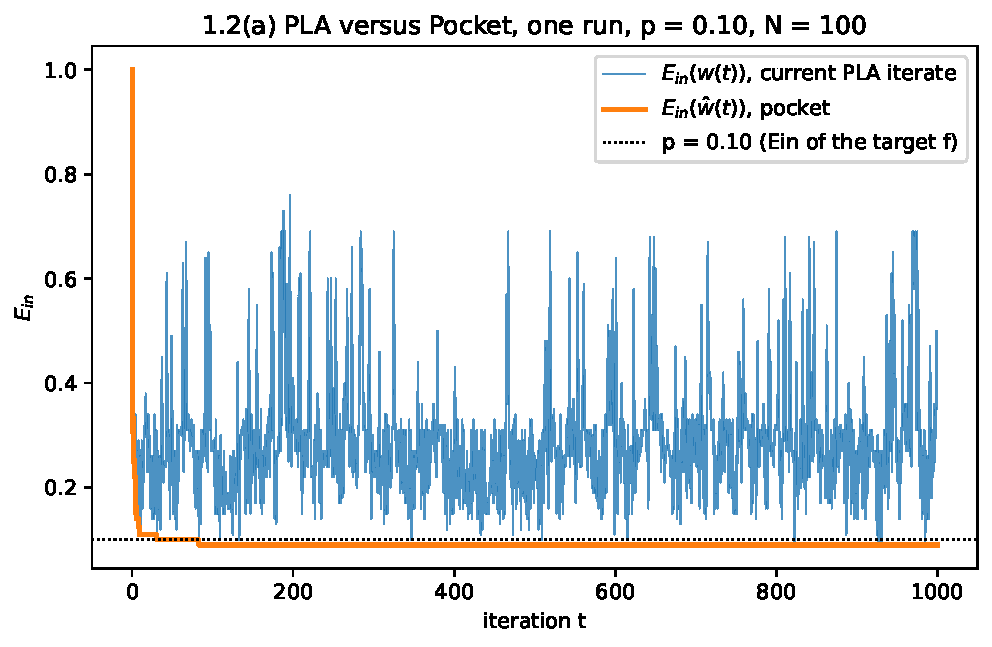
\includegraphics[width=0.255\textwidth]{fig_1_2a_ein_curves}\label{fig:p1a}}\hfil
\subfloat[]{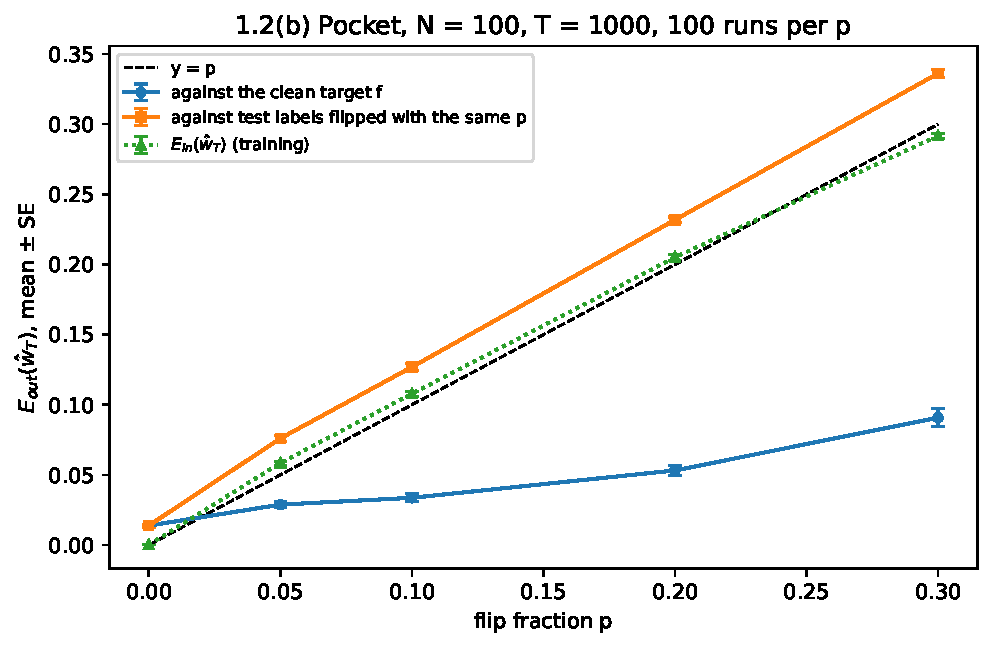
\includegraphics[width=0.255\textwidth]{fig_1_2b_eout_vs_p}\label{fig:p1b}}\hfil
\subfloat[]{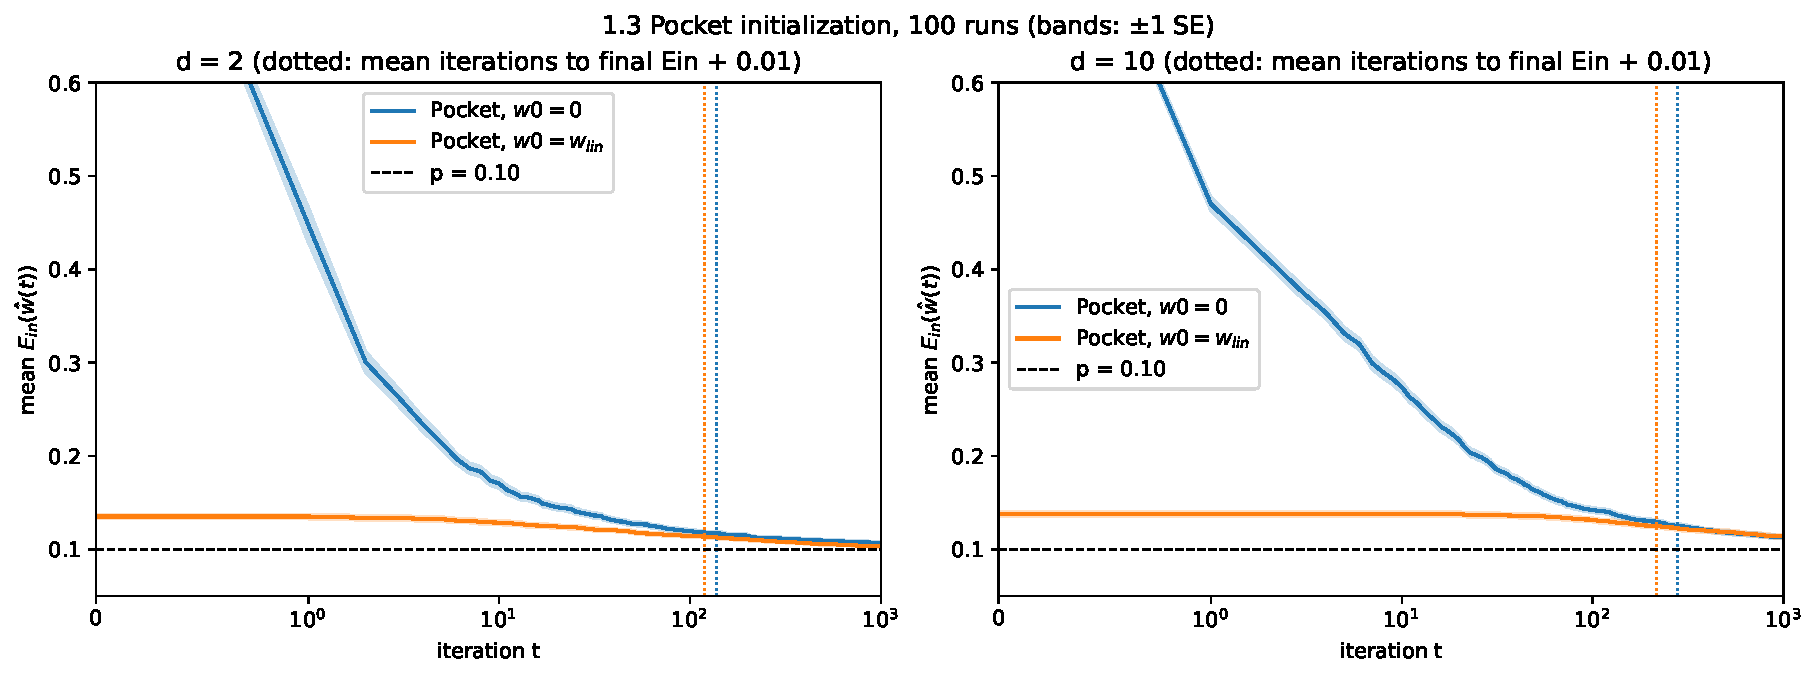
\includegraphics[width=0.47\textwidth]{fig_1_3_init}\label{fig:p1c}}
\caption{Part 1. (a) One run with $p=0.10$: the PLA iterate jumps, while Pocket's $\Ein(\hat\w(t))$ falls and ends below the target's own 0.10. (b) $\Eout(\hat\w_T)$ against the flip rate, measured against the clean $f$ and against flipped test labels, 100 runs per $p$. (c) Pocket started at $\w_0=0$ and at $\wlin$, $d=2$ and $d=10$, 100 runs (bands: $\pm1$ SE).}
\label{fig:p1}
\end{figure*}

\textbf{Simulated data (1.2).} How PLA acts with noisy labels and how quickly it converges when the data are separable. In the first case, when the flipped labels are 10\%, the data becomes noisy and no longer separable. Thereby, PLA does not converge, and its last iterate ends at a training error of 0.35. On the other hand, pocket achieves the best error of 0.09, slightly below the 0.10 of the target itself (Fig.~\ref{fig:p1}(a)).

Across 100 runs, the learned boundaries keep the accuracy as close to results with clean labels. The error with clean labels is $0.034\pm0.003$ for $p=0.10$ and $0.091\pm0.007$ for $p=0.30$. However, when the test labels are flipped in the same way, the error rises to $0.127\pm0.002$ and $0.336\pm0.003$ respectively (Fig.~\ref{fig:p1}(b)). It cannot fall below $p$, because a flipped test label is wrong exactly where the model agrees with $f$, and the expected error is described as: $E_{\mathrm{out}}^{\mathrm{flip}}=p+(1-2p)E_{\mathrm{out}}^{\mathrm{clean}}$.

\textbf{Convergence (1.2(c)).} The number of training points is important in terms of how fast PLA reaches $E_{\mathrm{in}}=0$. With a limit of $T=1000$ updates over 500 runs, almost all runs converge for $N=100$, within $0.4\%\pm0.3\%$ failures, but the failure rate increased up to $21.4\%\pm1.8\%$ with $N=1000$. Since the larger datasets become, there are more points close to decision boundary, which makes the median bound $R^2\lVert\mathbf{w}^*\rVert^2/\rho^2$ increase from $7.3\times10^4$ to $6.8\times10^6$. The converged runs required a median of only 58 and 421 updates, even though the bound is greater than $T$, which is a worst case scenario for theoretical bound.

\textbf{Initialization (1.3).} Started at $\wlin$, Pocket begins at $\Ein\approx0.14$ instead of 1 (Fig.~\ref{fig:p1}(c)), so it needs fewer iterations to come within 0.01 of its final $\Ein$ (an absolute tolerance, since 1\% of 0.1 is below the $1/N$ resolution). It needs $119\pm18$ against $137\pm18$ for $d=2$, and $216\pm25$ against $278\pm23$ for $d=10$. The saving grows with $d$, from 18 to 62 iterations, because PLA builds its direction one point at a time while $\wlin$ costs one least-squares solve for any $d$. The final $\Ein$ is almost the same from both starts (0.1035 and 0.1072 for $d=2$), since the first PLA updates move away from $\wlin$ and only the stored pocket weights keep the advantage.

\begin{figure}[!t]
\centering
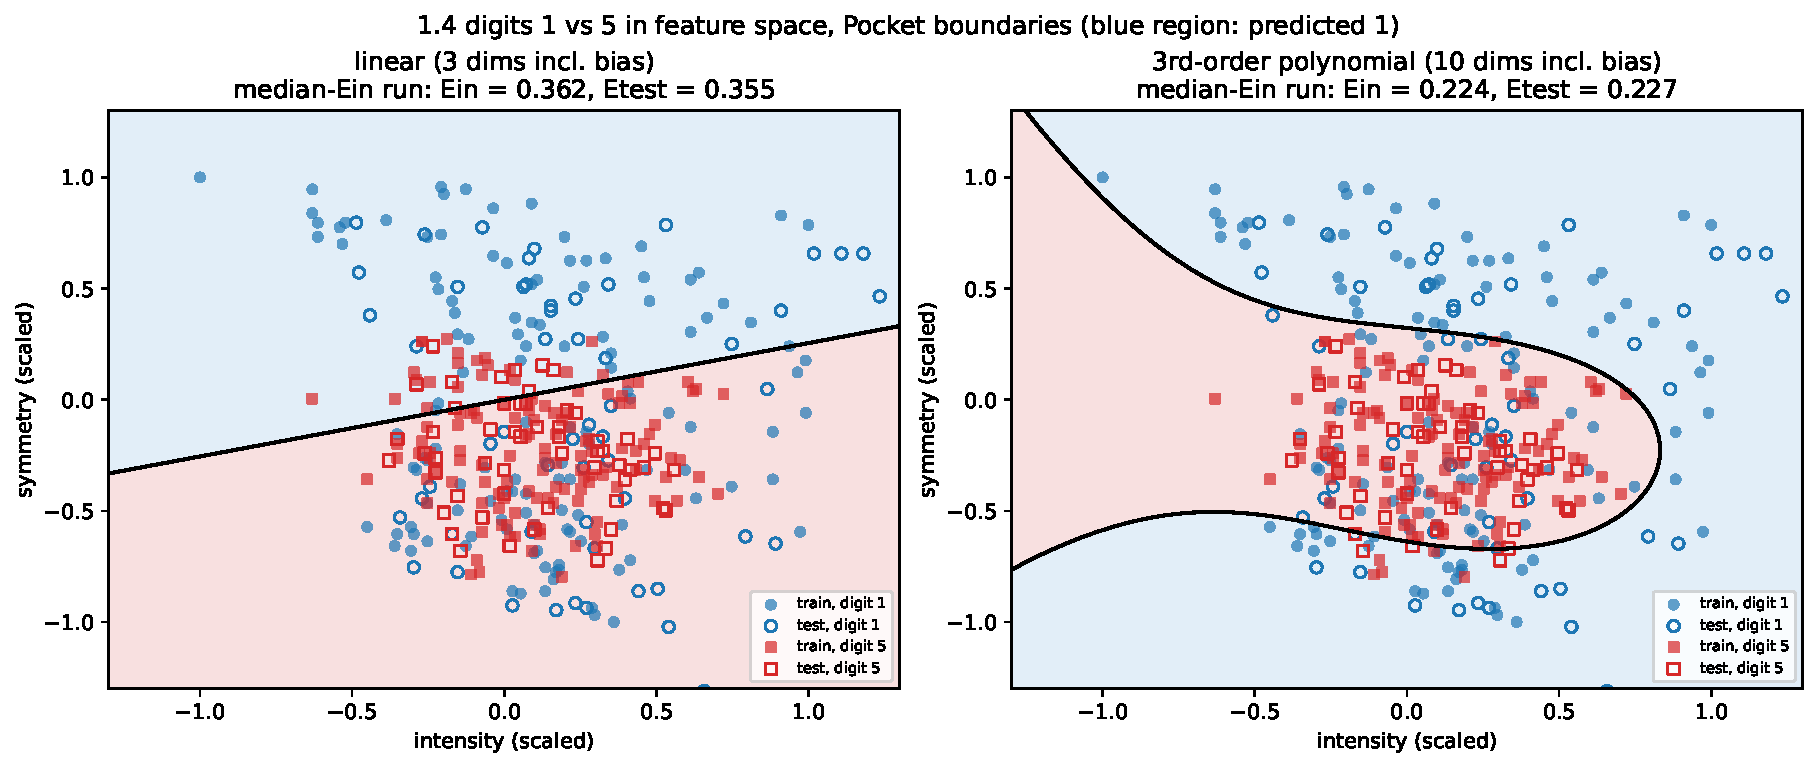
\includegraphics[width=0.85\columnwidth]{fig_1_4_boundaries}
\caption{Digits 1 vs 5 (\texttt{load\_digits}) in the scaled intensity--symmetry plane, with the Pocket boundary of the median-$\Ein$ run for linear (left) and third-order polynomial (right) features.}
\label{fig:p1d}
\end{figure}

\textbf{Digits (1.4).}
Original images are $8\times8$ pixel images from \texttt{load\_digits} dataset. Digits 1 and 5 are classified via 2 features scaled to $[-1,1]$ with training statistics, the one is intensity, focusing on the brightness of the digit picture, the second is the symmetry test (Fig.~\ref{fig:p1d}). Data divided into 70/30, having 70\% as training set, and 30\% as test set.

After 100 pocket runs, the linear model reached $E_{\mathrm{in}}=0.357\pm0.001$ on training set and $E_{\mathrm{test}}=0.352\pm0.002$ on test data. Whereas, cubic model, which had transformed feature, such as nonlinear combinations, decreased the error to $E_{\mathrm{in}}=0.222\pm0.0004$ and $E_{\mathrm{test}}=0.2065\pm0.0011$ respectively.

Regarding the generalization bound, for 110 test points, the Hoeffding margin of 95\% is $\epsilon=0.129$. The resulting upper bounds are $E_{\mathrm{out}}\le0.484$ for linear model and $E_{\mathrm{out}}\le0.357$ for cubic model. When $M=2$ models are considered together, the margin increases to $\epsilon=0.141$, because the probability applies to both models. The VC terms on 254 training points are 0.85 for $d_{\mathrm{VC}}=3$ and 1.45 for $d_{\mathrm{VC}}=10$. It represents the complexity of models, meaning that the cubic model is more flexible, so its complexity penalty is larger.  We trust the cubic model more, because its test bound is lower and its $E_{\mathrm{test}}$ shows no gap from $E_{\mathrm{in}}$. Pocket itself only guarantees a low $E_{\mathrm{in}}$, so any claim about $E_{\mathrm{out}}$ has to come from a bound like this.

\subsection{Part 2: Linear regression}
\begin{figure*}[!t]
\centering
\subfloat[]{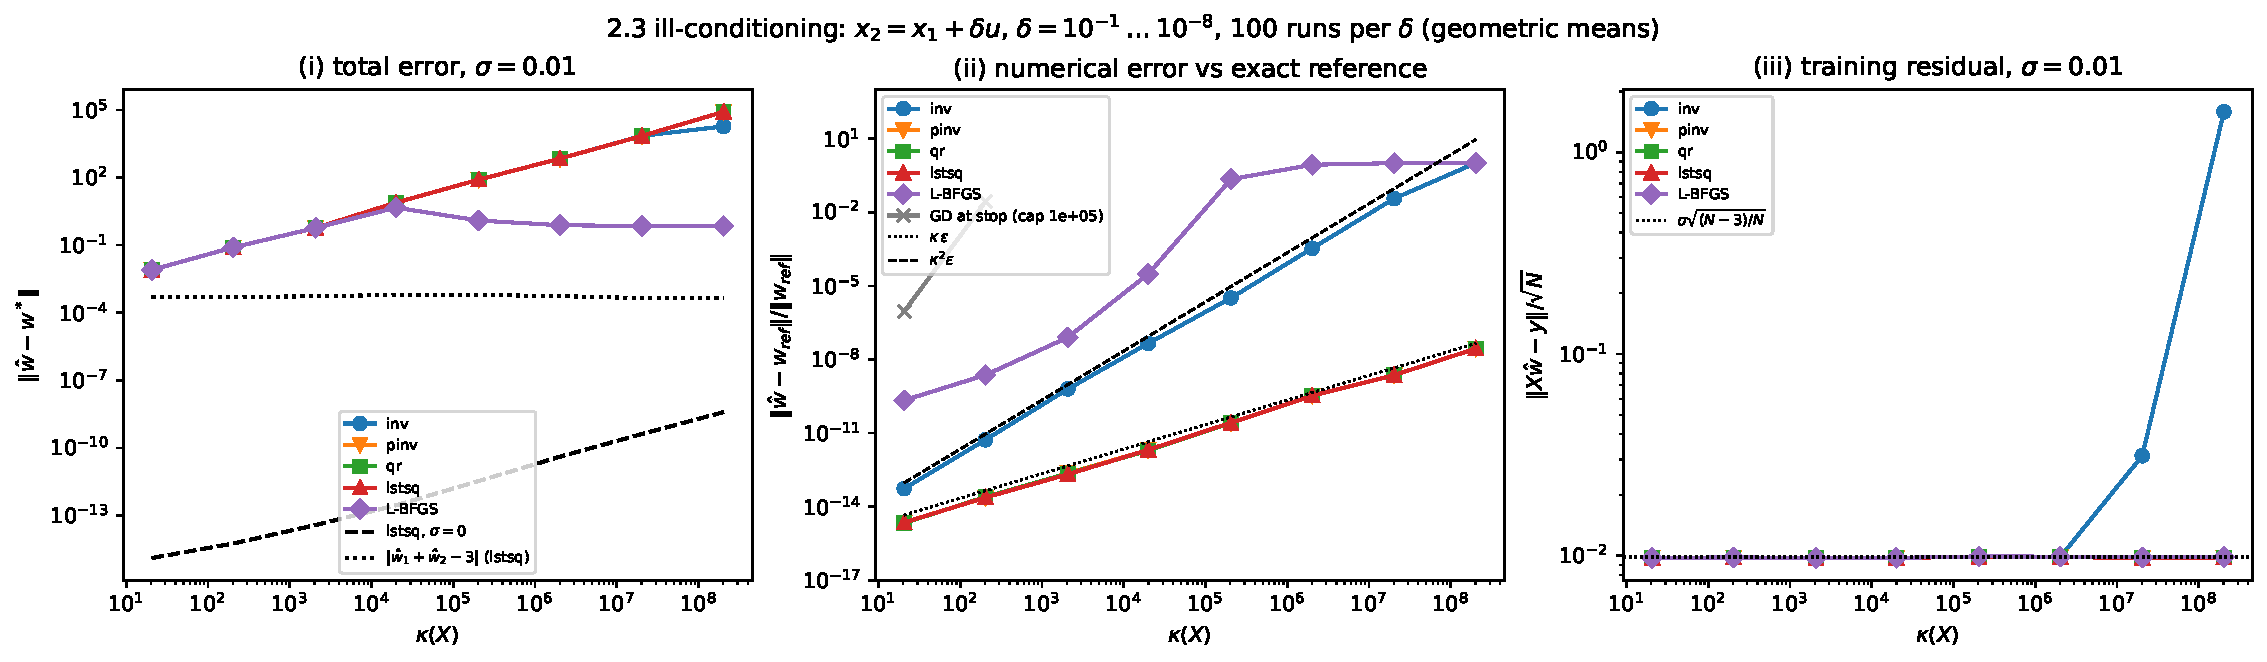
\includegraphics[width=0.53\textwidth]{fig_2_3_coef_error}\label{fig:p2a}}\hfil
\subfloat[]{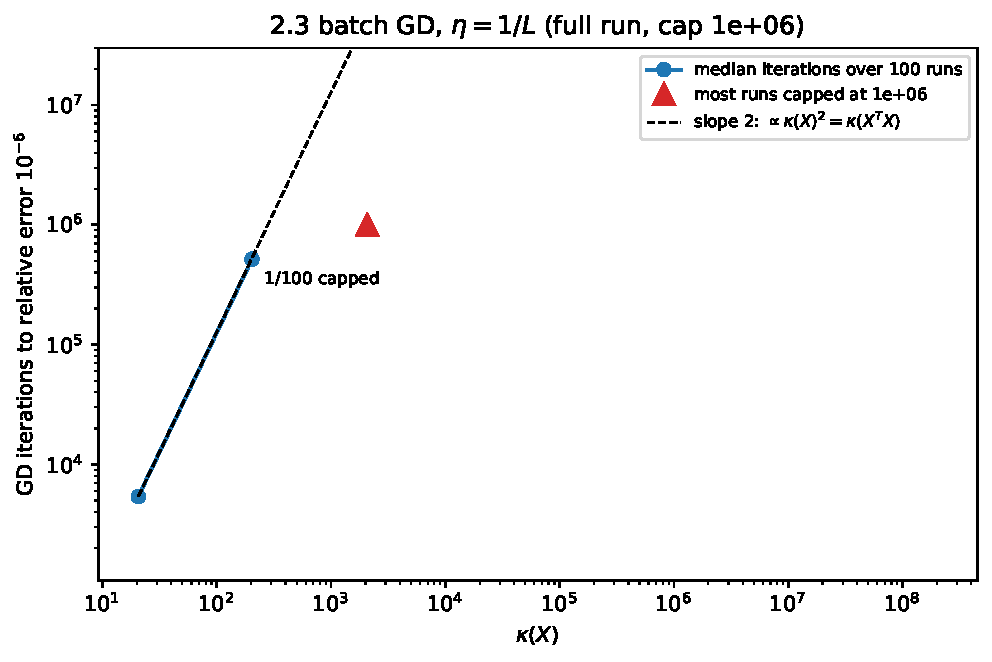
\includegraphics[width=0.255\textwidth]{fig_2_3_gd_iterations}\label{fig:p2b}}\\
\subfloat[]{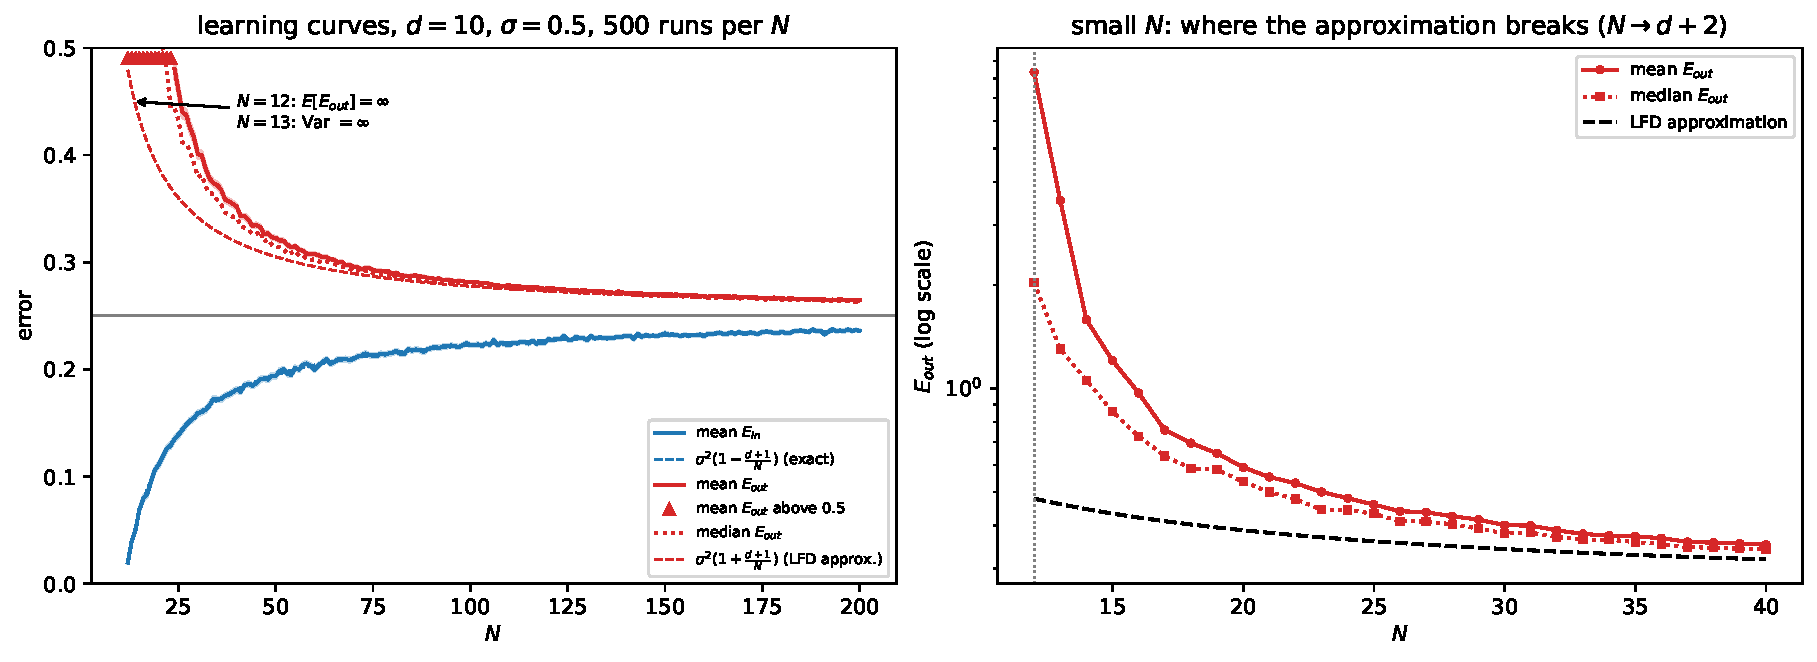
\includegraphics[width=0.43\textwidth]{fig_2_4_learning_curves}\label{fig:p2c}}\hfil
\subfloat[]{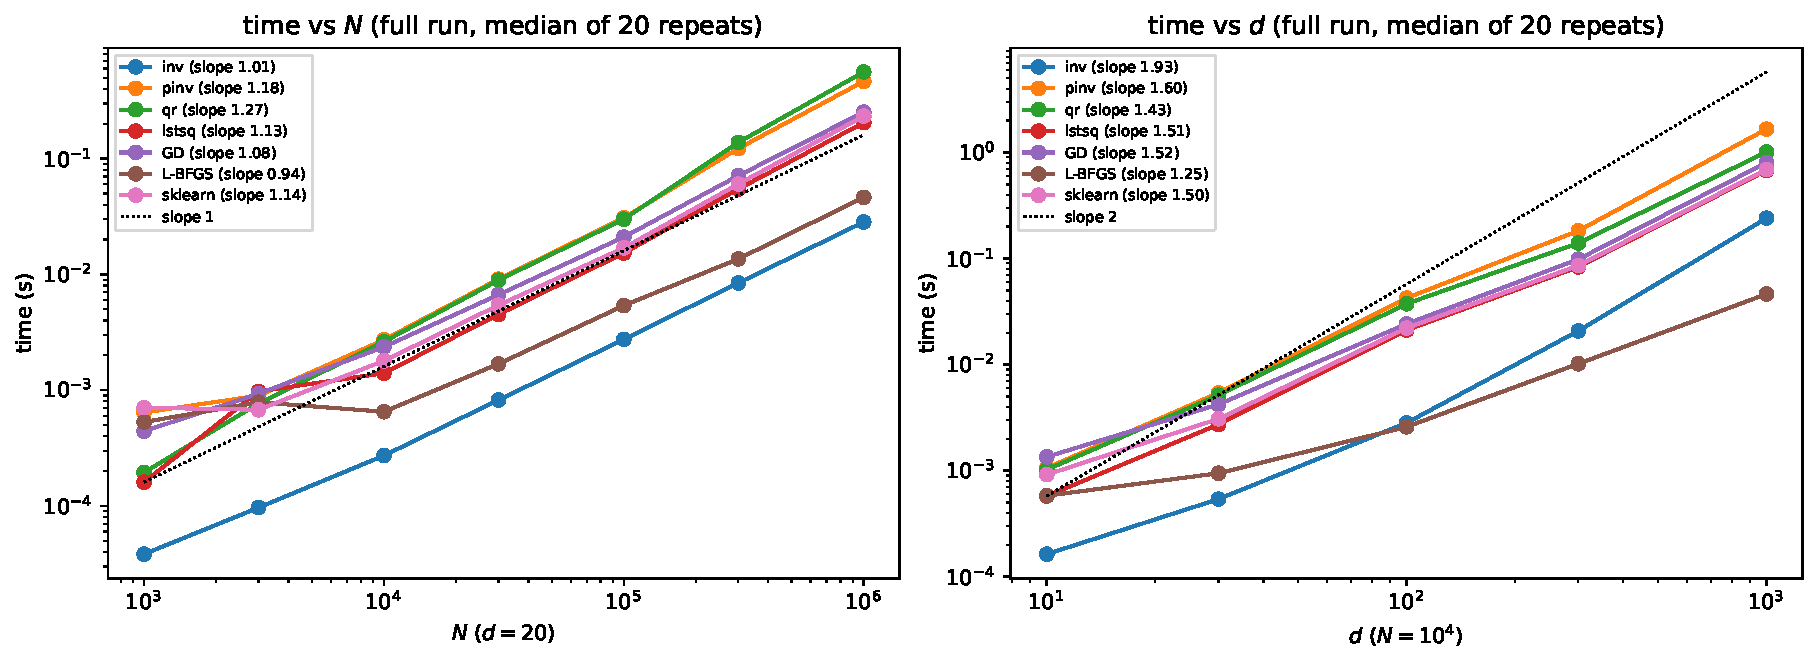
\includegraphics[width=0.43\textwidth]{fig_2_6_timing}\label{fig:p2d}}
\caption{Part 2. (a) Coefficient error and residual of the five solvers against $\kappa(\X)$ (100 runs per $\delta$). (b) Gradient-descent iterations to a relative error of $10^{-6}$ against $\kappa(\X)$. (c) Learning curves, $d=10$, 500 runs per $N$, with LFD's formulas. (d) Solver timing against $N$ ($d=20$) and $d$ ($N=10^4$), single BLAS thread, median of 20 repeats.}
\label{fig:p2}
\end{figure*}

\textbf{Solvers and conditioning (2.2, 2.3).}
This part focuses on the correctness of gradient and regression solvers.

The analytical gradient is likely to be correct, since gradient check gives an error of $3.4\times 10^{-10}$, which is relatively small. Considering five solvers, the solutions varies from lstsq's one by around $1.4\times 10^{-9}$, meaning that the solvers agree up to their tolerances.

Eventually, there is second feature in a form of $x_2=x_1+\delta u$. In case the value of $\delta$ is $10^{-1}$, the condition number is only 21. The condition is increased, to make $x_2$ as close to $x_1$, by putting $\delta=10^{-8}$, so the condition is $2\times 10^8$. It is the evidence that the problem is sensitive. As for numerical error, QR, SVD, and lstsq have errors approximately about $2.8\times 10^{-8}$ (Fig.~\ref{fig:p2}(a)). The direct inverse method is less stable since it begins computations with $X^TX$. The condition number is squared, so that its error rises as $\kappa^2\epsilon_{\mathrm{mach}}$, and with $\kappa=2\times 10^8$ it reaches 100\%. It is assumed that the ultimate solution is unreliable, and the problem is ill-conditioned with respect to numerical progress. Gradient descent needs about $\kappa^2$ iterations: 5\,400 at $\kappa=20.6$ and 516\,600 at $\kappa=203$ (Fig.~\ref{fig:p2}(b)). L-BFGS stalls from $\kappa\approx2\times10^5$. We would ship QR or \texttt{lstsq}, because the lecture formula squares $\kappa$ before solving.

\textbf{Learning curves (2.4).}

Main idea is to analyze the error change, when the training examples $N$ increases. The $E_{\mathrm{in}}$ formula holds over 189 values of $N$ (Fig.~\ref{fig:p2}(c)). Its parameters: deviation is only 2.7 standard errors, median deviation is 0.5. The approximation for the expected test error $E_{\mathrm{out}}$ is less accurate. It underestimates the result by 18 standard errors when $N=20$ and still underestimates it by 3.6 standard errors when $N=200$. The problem is when $N$ is close to $d+1$, because there are almost as many parameters as data points.

In case it is $N=12$ the mean $E_{\mathrm{out}}=8.3 \pm 2.1$ while the value of median 2.0. Again, the problem is that the approximation fails because the expected inverse matrix grows approximately like $1/(N-d-2)$, not simply like $1/N$.

\textbf{California housing (2.5).}

The model uses 16512 data points and 9 weights. The training MSE is 0.527 and test MSE is $0.515\pm0.018$, with test $R^2=0.605$. Due to insignificant differences of MSE, it is apparent that there is no sign of overfitting.

The target is capped at \$500\,000 for 5\% of districts, and the model is on average 1.08 below these values. According to the results, the standardized values are about $-0.91$ for latitude, $-0.88$ for longitude and $+0.83$ for income. The advantage of standardization in such cases is that the coefficients could be compared more straightforward as the features are on similar scale. The covariation between longitude and latitude ($-0.93$) conveys the locational information, so their individual coefficients should not be interpreted separately.

\textbf{Timing (2.6).} In $N$ every solver scales with slope 0.94--1.27, consistent with $O(Nd^2)$ for the direct methods (Fig.~\ref{fig:p2}(d)). In $d$ only \texttt{inv} reaches the predicted slope 2 (1.93); the others reach 1.25--1.60, because BLAS-3 kernels become more efficient as matrices grow. \texttt{inv} is also the fastest at $N=10^6$ (0.028\,s, against 0.20\,s for \texttt{lstsq}), but 2.3 shows that it is the least accurate.

\textbf{Linear regression for classification (2.7).} On the 1.4 digits, $\mathrm{sign}(\wlin\T\x)$ has $\Ein=0.421$ against Pocket's $0.355$. Squared loss also penalizes correct points far from the boundary, so the fitted line sits between the two groups of 1s. It is still a useful starting point, and Pocket from $\wlin$ ends at $\Ein=0.349$ and $E_{\mathrm{test}}=0.340$.

\subsection{Part 3: Logistic regression}
\begin{figure*}[!t]
\centering
\subfloat[]{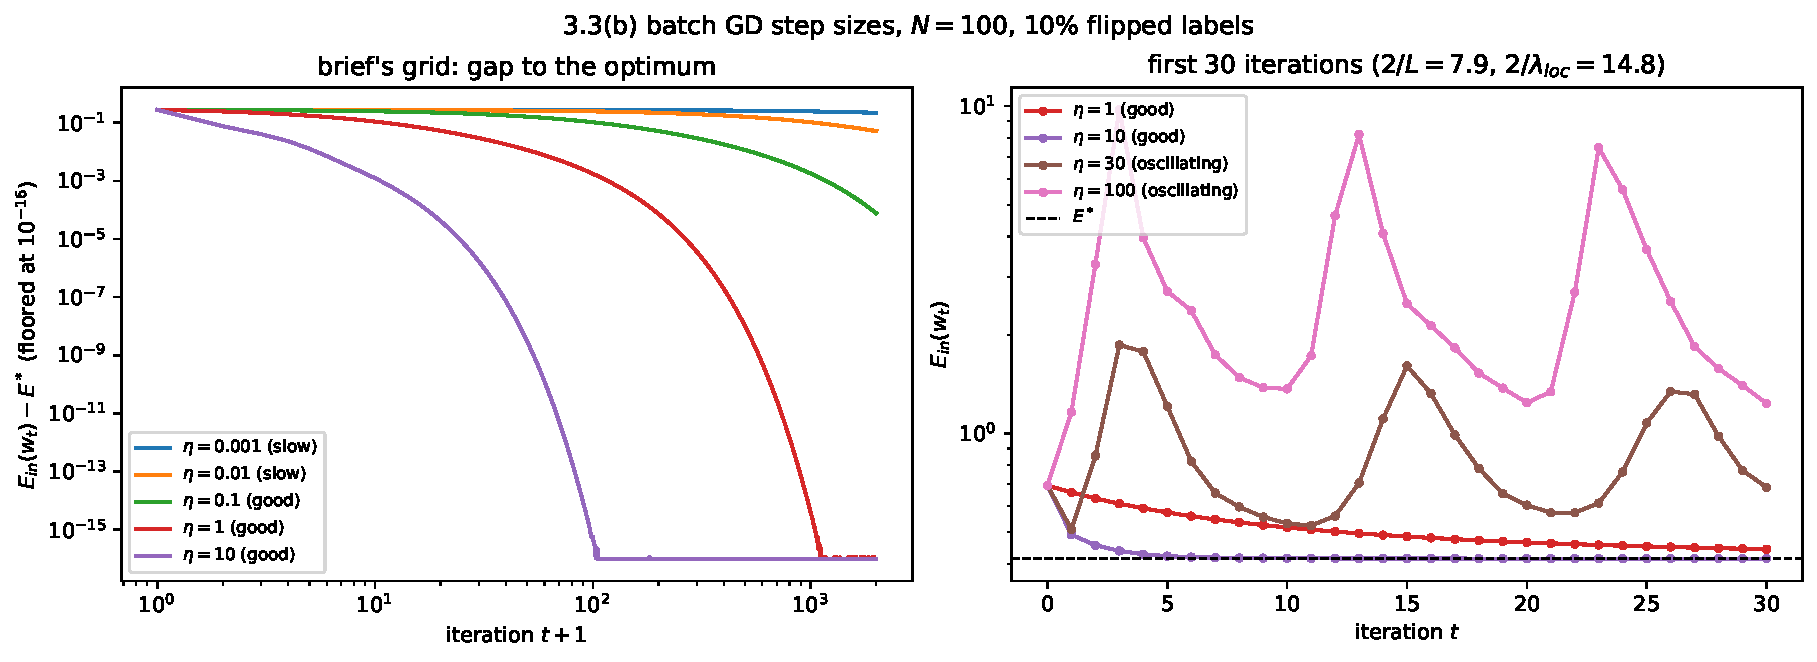
\includegraphics[width=0.43\textwidth]{fig_3_3b_step_sizes}\label{fig:p3a}}\hfil
\subfloat[]{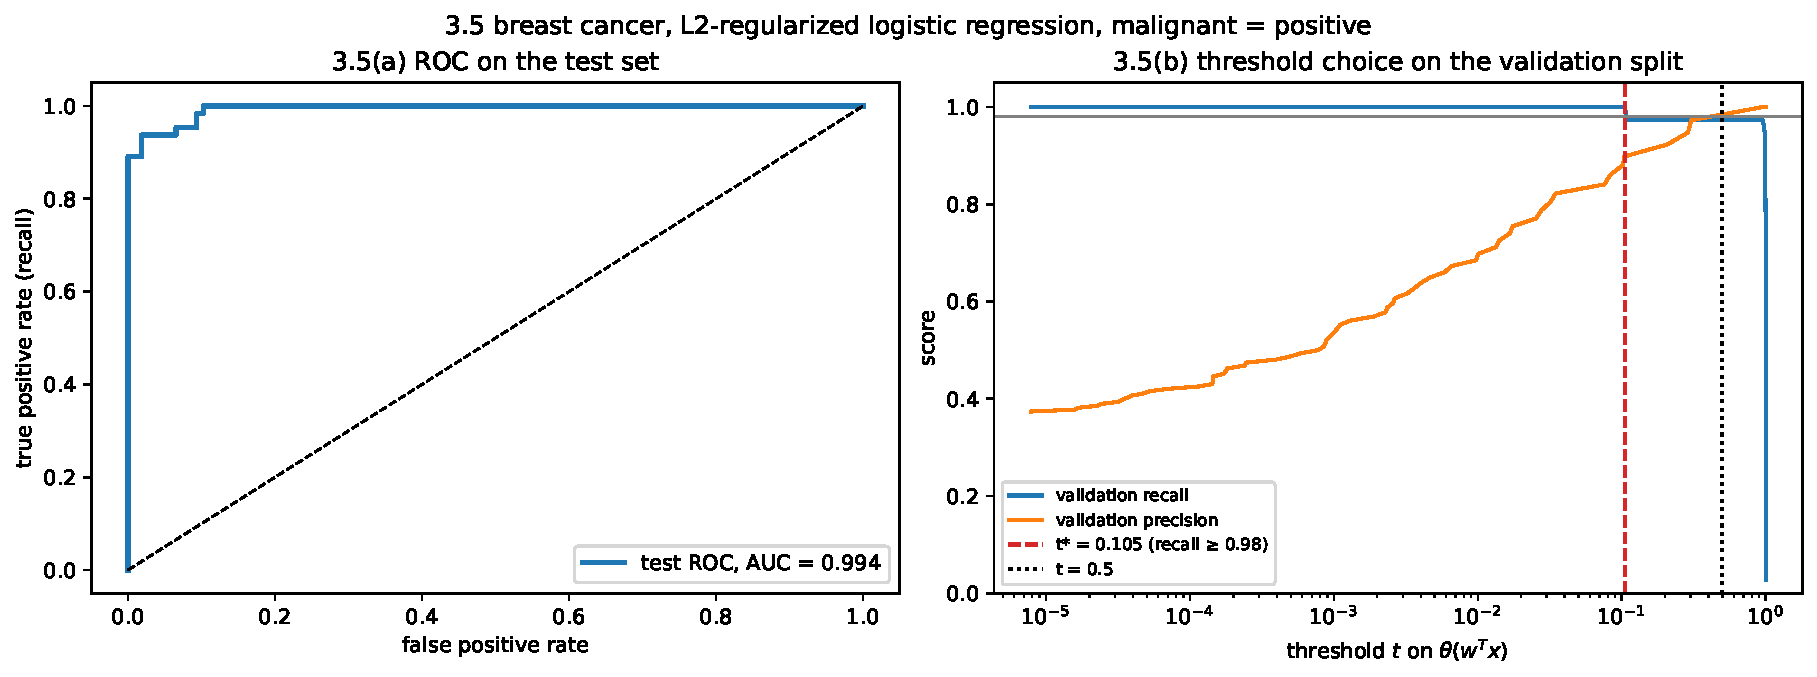
\includegraphics[width=0.43\textwidth]{fig_3_5_roc_threshold}\label{fig:p3b}}\\
\subfloat[]{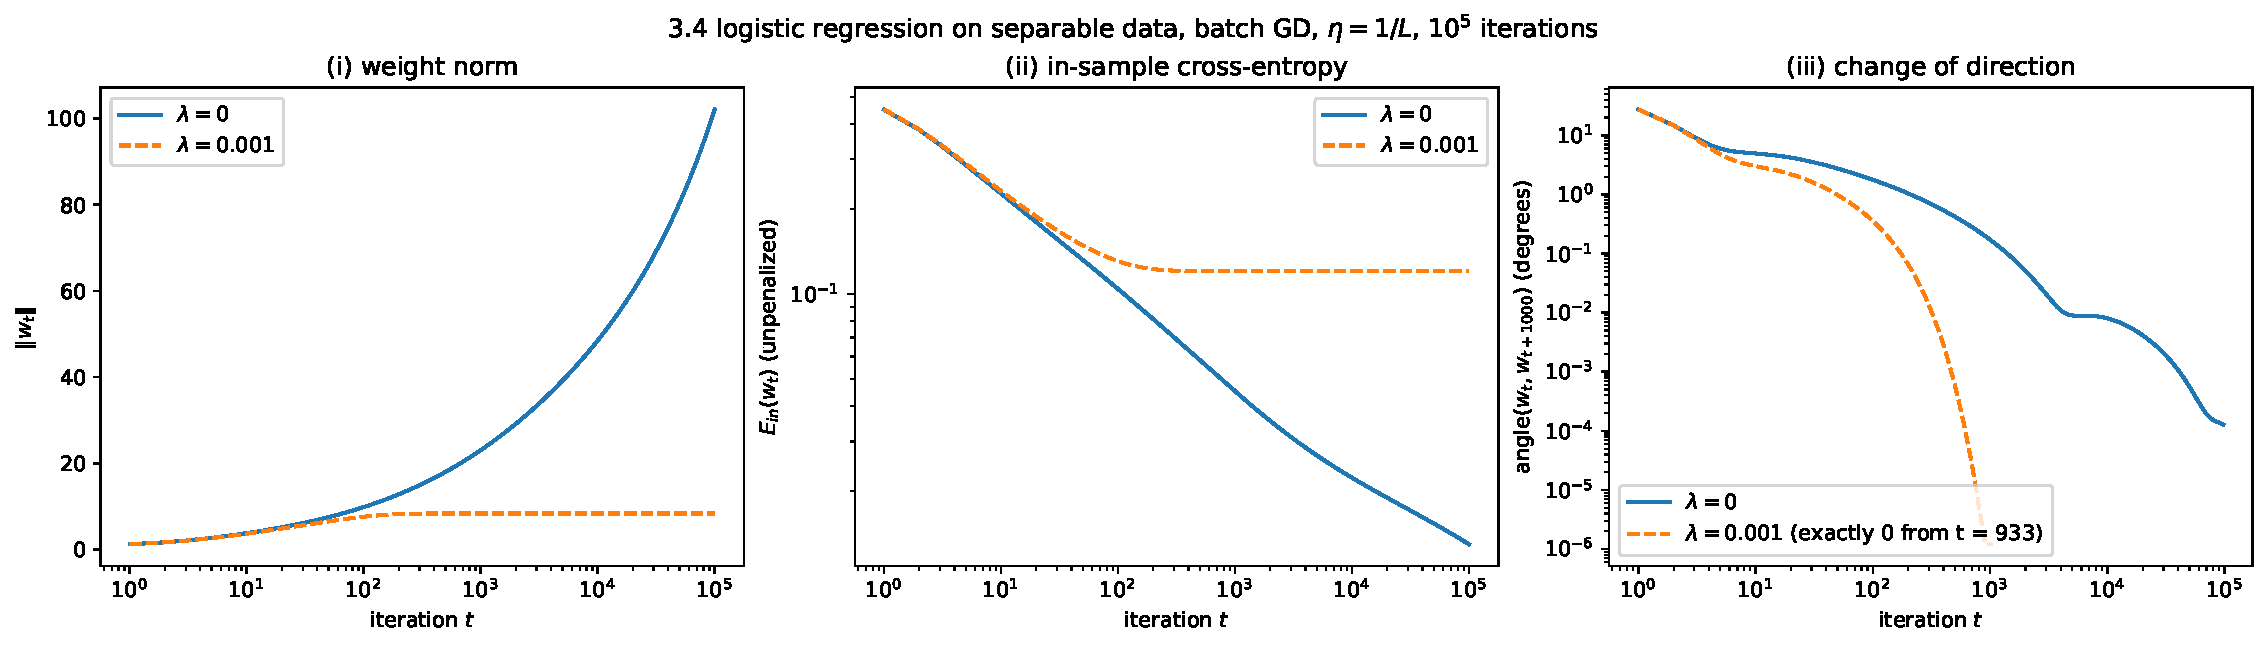
\includegraphics[width=0.45\textwidth]{fig_3_4_separable}\label{fig:p3c}}
\caption{Part 3. (a) Batch GD on noisy data for $\eta$ from $10^{-3}$ to 100. (b) Breast cancer: test ROC and the choice of a recall-$\ge0.98$ threshold on a validation split. (c) Separable data: $\lVert\w_t\rVert$, $\Ein(\w_t)$ and the angle between $\w_t$ and $\w_{t+1000}$, without and with L2 ($\lambda=10^{-3}$).}
\label{fig:p3}
\end{figure*}

\textbf{Stability and optimizers (3.2, 3.3).} At $s=\pm1000$ the stable $\Ein$ returns exactly 500 with no warnings, where the naive formula overflows to \texttt{inf}. With $\eta=0.01$ and the brief's stopping rule, SGD needs $333\pm5$ epochs and reaches a cross-entropy $\Eout$ of $0.102\pm0.001$ (100 runs). To give the optimum a finite value, we flip 10\% of the labels for the step-size sweep (Fig.~\ref{fig:p3}(a)). After 2\,000 iterations, $\eta\le10^{-2}$ is still 0.05--0.22 above $E^*$ (slow), $\eta=1$ and $10$ have converged (good), and $\eta=30$ and $100$ oscillate, with 992 and 597 increases of $\Ein$. $\eta=10$ exceeds the global bound $2/L=7.9$ but not the local one at the optimum, $2/\lambda_{\max}(\nabla^2\Ein(\w^*))=14.8$. To reach $E^*+10^{-6}$, L-BFGS needs 11 iterations (about 0.3\,ms) and gradient descent 31 at $\eta=10$ (about 0.3\,ms). SGD needs 344 epochs at $\eta=0.01$ (about 0.1\,s) and 1\,494 at $\eta=0.1$ (about 0.45\,s). With a constant step, SGD's gradient noise sets a floor that grows with $\eta$, so the larger step is slower.

\textbf{Separable data (3.4).} 
Without regularization, $\lVert \mathbf{w}_t\rVert$ grows from 23 to 102 during $10^5$ iterations, $E_{\mathrm{in}}$ decreases from 0.045 to 0.013, since normally models increase the weight vector so that all the probabilities approach 0 or 1, in case when training points are on the correct side of the decision boundary. Also the angle between $\mathbf{w}_t$ and $\mathbf{w}_{t+1000}$ reduces from 0.17 to $1.3\times10^{-4}$ degrees: the direction converges to the max-margin separator~\cite{soudry2018}, even though the weights keep growing. Adding an L2 penalty changes the situation because the objective now includes a cost for large weights, $E_{\mathrm{in}}(\mathbf{w})+\lambda\lVert\mathbf{w}\rVert^2$: with $\lambda=10^{-3}$ the norm stops at 8.37 and $E_{\mathrm{in}}$ at 0.120 (Fig.~\ref{fig:p3}(c)), as the model balances small weights against fitting the training points.

\textbf{Breast cancer (3.5).}
In this experiment, logistic regression is used for classification of tumors as malignant (represented by target 0). The data is split into 70/30, as done in other parts. The training data are linearly separable, so the weights may never converge to the finite optimum, hence the addition of $L_2$ regularization, with $\lambda^*=1.8\times10^{-3}$ chosen by 10-fold CV. However, there are still 6 of the 64 malignant tumors that are incorrectly classified as non-cancerous, which is important false-negative rate. To lower the rate of false negative predictions, a lower threshold $t^*=0.105$ is chosen from the validation data, where the minimum required recall is 0.98. At threshold 0.5 the model yields an accuracy of 0.953, a precision of 0.967, a recall of 0.906, $F_1=0.936$, and an AUC of 0.994; at the new threshold the test recall rises to 0.953 and the precision falls to 0.859. There are only 37 malignant cases in the validation set, causing this threshold selection to be sensitive (of 37 cases, one is missed, so it is 0.027). There is a higher percentage of cases detected as malignant, plus 9 extra false alarms (Fig.~\ref{fig:p3}(b)). So, for this problem, the threshold 0.5 is not always the best choice, since it is worse to miss a cancer diagnosis than it is to have to conduct another exam.

\subsection{Part 4: Overfitting and regularization}
\begin{figure*}[!t]
\centering
\subfloat[]{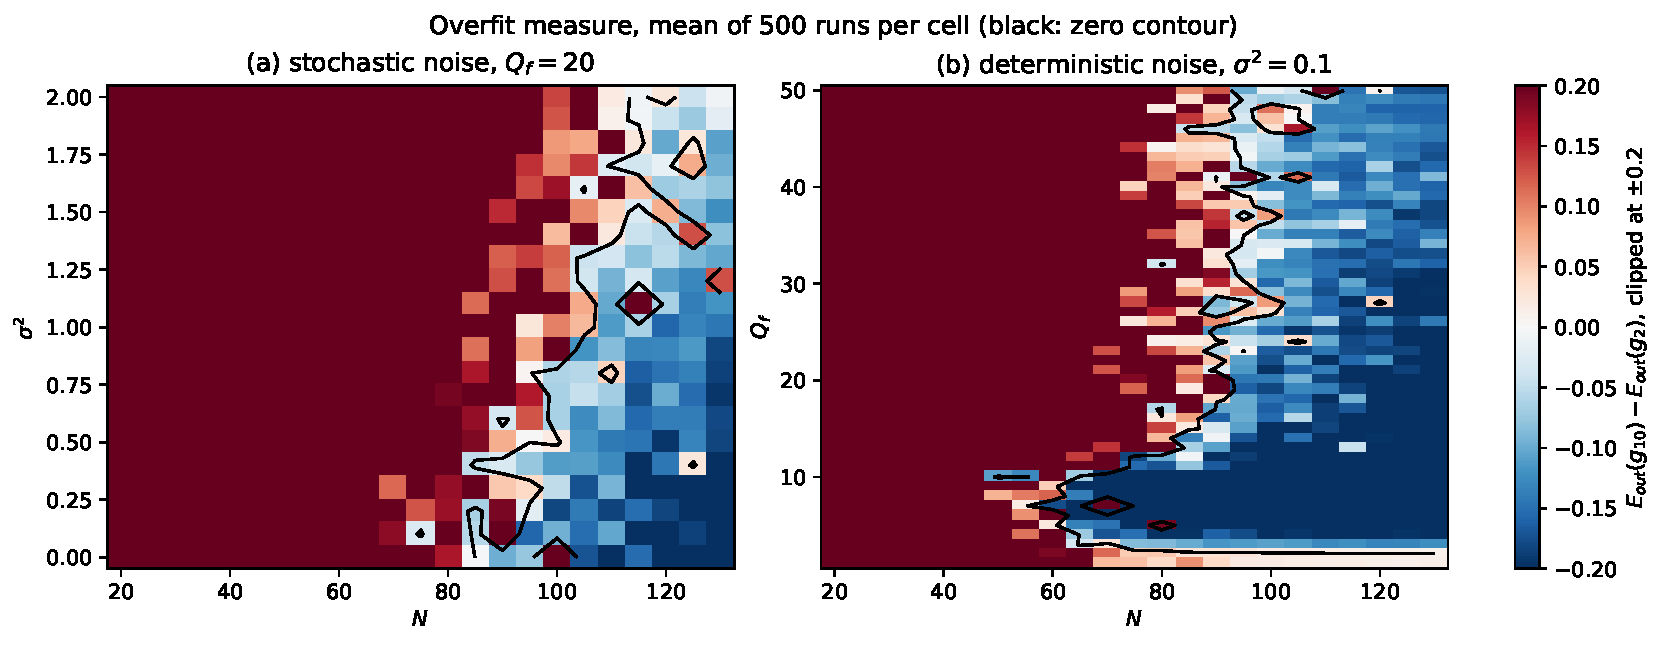
\includegraphics[width=0.52\textwidth]{fig_4_1c_heatmaps}\label{fig:p4a}}\\
\subfloat[]{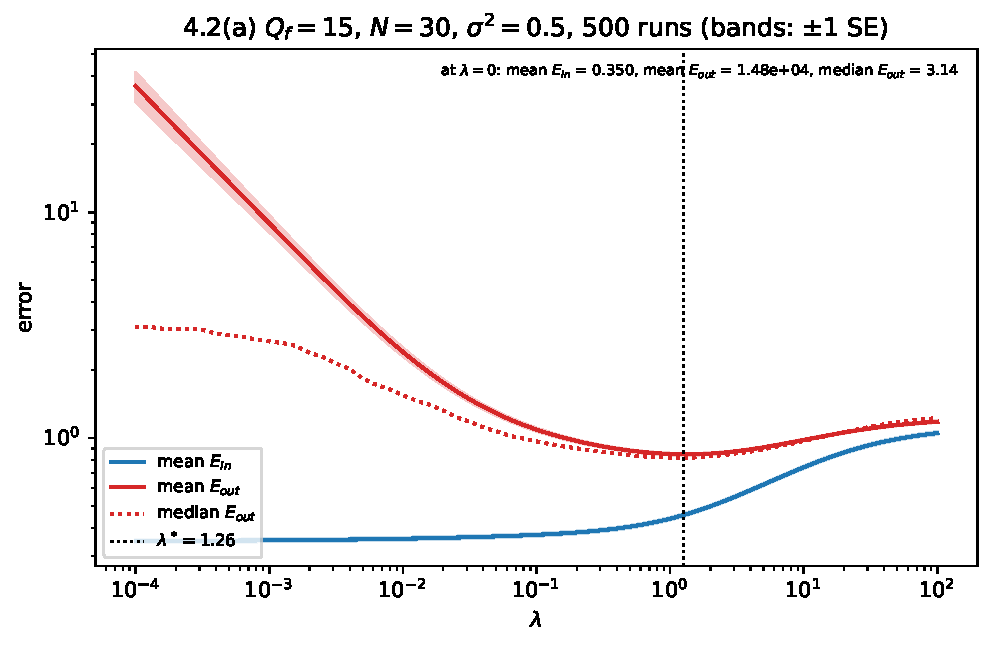
\includegraphics[width=0.29\textwidth]{fig_4_2a_lambda_sweep}\label{fig:p4c}}\hfil
\subfloat[]{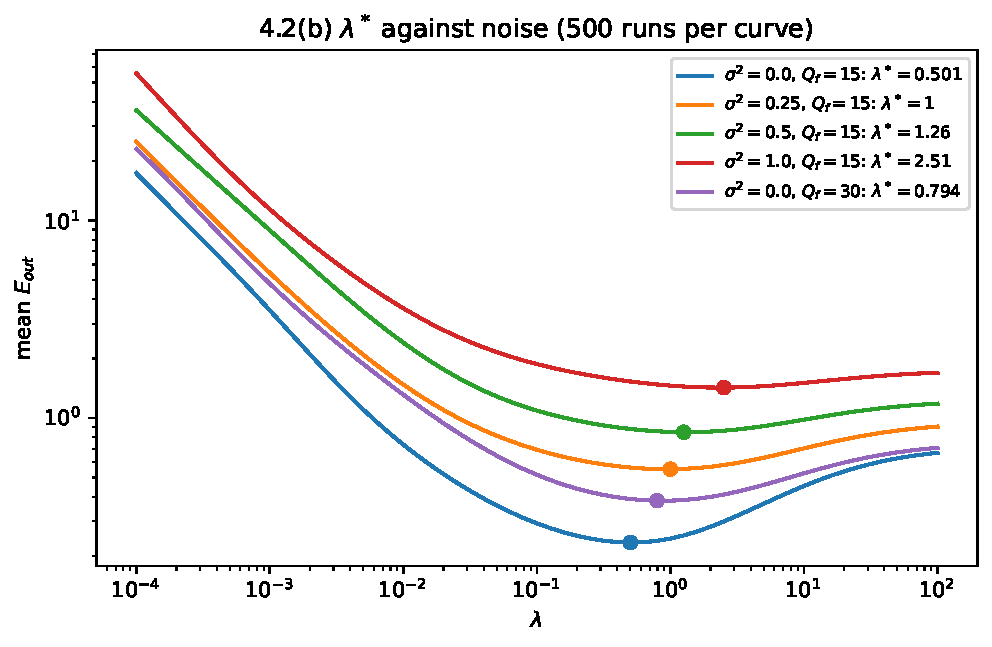
\includegraphics[width=0.29\textwidth]{fig_4_2b_noise_lambda_star}\label{fig:p4d}}\hfil
\subfloat[]{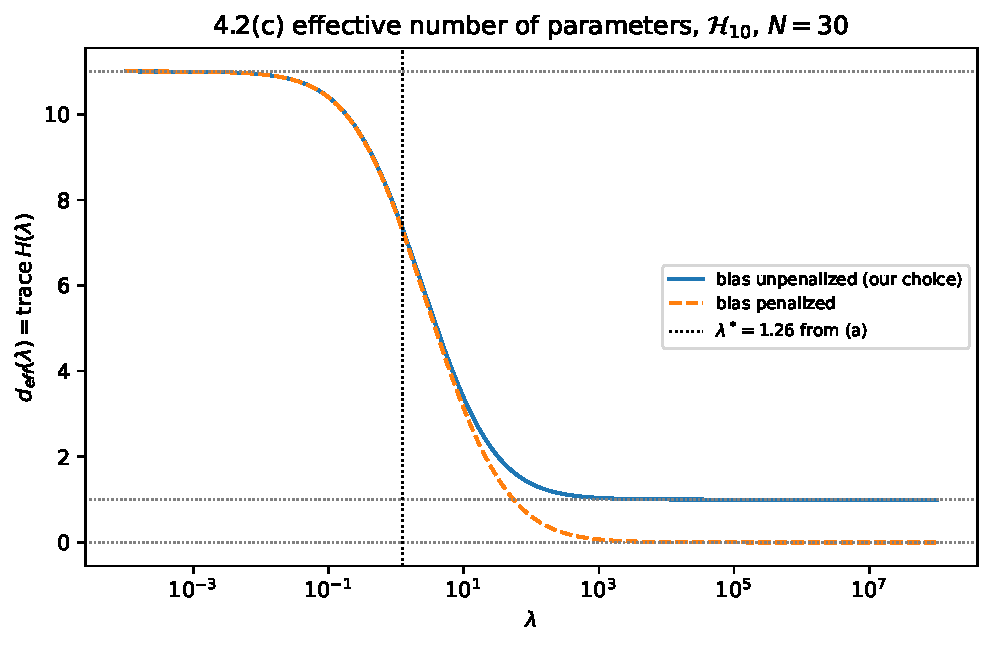
\includegraphics[width=0.29\textwidth]{fig_4_2c_deff}\label{fig:p4e}}
\caption{Part 4. (a) Overfit measure $\Eout(g_{10})-\Eout(g_2)$ against $N$ and $\sigma^2$ ($Q_f=20$), and against $N$ and $Q_f$ ($\sigma^2=0.1$), with 500 runs per cell and analytic $\Eout$. (b) Weight decay, $Q_f=15$, $N=30$, $\sigma^2=0.5$, 500 runs. (c) $\Eout(\lambda)$ for four noise levels and the deterministic case. (d) $d_{\mathrm{eff}}(\lambda)$.}
\label{fig:p4}
\end{figure*}

\textbf{Overfitting (4.1).} We used $\Eout(g_{10})-\Eout(g_2)$ with the analytic formula \eqref{eq:eout} to measure overfitting with 500 runs per cell. It changes sign at the overfitting boundary, and when it is positive, the degree-10 model overfits. The heatmaps in Fig.~\ref{fig:p4}(a) show the effect of stochastic noise $\sigma^2$ with $Q_f=20$ and deterministic noise $Q_f$ with $\sigma^2=0.1$ on the boundary. The position of the boundary, at which the median changes sign, is shifted from $N=40$ ($\sigma^2=0$) to $N=95$ ($\sigma^2=2$) by stochastic noise. This means that models with lots of features, like $g_{10}$, require more data to take advantage of their flexibility. Deterministic noise pushes the boundary to larger $N$ as well, moving it from $N=30$ when $Q_f=10$ to 40 when $Q_f=20$ and 55 when $Q_f=50$.
If $\sigma^2$ is small, $\mathcal H_{10}$ tries to fit the part of $f$ above degree 10, which it cannot represent. At 20--50 random points, $L_{11},\dots,L_{Q_f}$ are not orthogonal to the low orders, so least squares aliases them into incorrect low-order coefficients and target complexity acts as noise. For $Q_f=2$ the target already lies in $\mathcal H_2$, so $\mathcal H_{10}$ overfits at every $N$, with $+0.010\pm0.001$ at $N=130$. Medians are reported because rare runs with $N$ near the 11 parameters oscillate wildly around $x=\pm1$: at $N=20$ the medians are 4 to 70, and 75\% of the cells have a positive mean but only 41\% a positive median.

\textbf{Weight decay (4.2).} As the penalty factor $\lambda$ grows, $\Ein$ rises, but $\Eout$ is U-shaped, with its minimum $0.848\pm0.008$ at $\lambda^*=1.26$ (Fig.~\ref{fig:p4}(b)). For $\lambda=0$, the mean $\Eout$ is $1.5\times10^4$, but the median is 3.14, which indicates a heavy tail from a few runs, and even a small $\lambda$ handles them due to \eqref{eq:ridge} using $s_i/(s_i^2+\lambda)$ instead of $1/s_i$.
Both noise types move $\lambda^*$ up (Fig.~\ref{fig:p4}(c)): as $\sigma^2$ increases from 0 to 1, $\lambda^*$ grows from 0.50 to 1.0, 1.26 and 2.51. Without stochastic noise it stays positive ($\lambda^*=0.79$ at $Q_f=30$), due to deterministic noise.
For larger values of $\lambda$, $d_{\mathrm{eff}}$ decreases from 11 to 7.30 at $\lambda^*$, then approaching 1, the constant $\bar y$ (Fig.~\ref{fig:p4}(d)). On one dataset, $\lambda=0$, 1.26 and 100 give $\Eout=8710$, 0.771 and 1.063: under-, well- and over-regularized.
There was no penalization applied to the bias since, for example, after shifting $y$ by 3, the penalized model degrades to $\Eout=6.66$, while the unpenalized one is unchanged. The method should not be specific to the origin of $y$.

\begin{figure*}[!t]
\centering
\subfloat[]{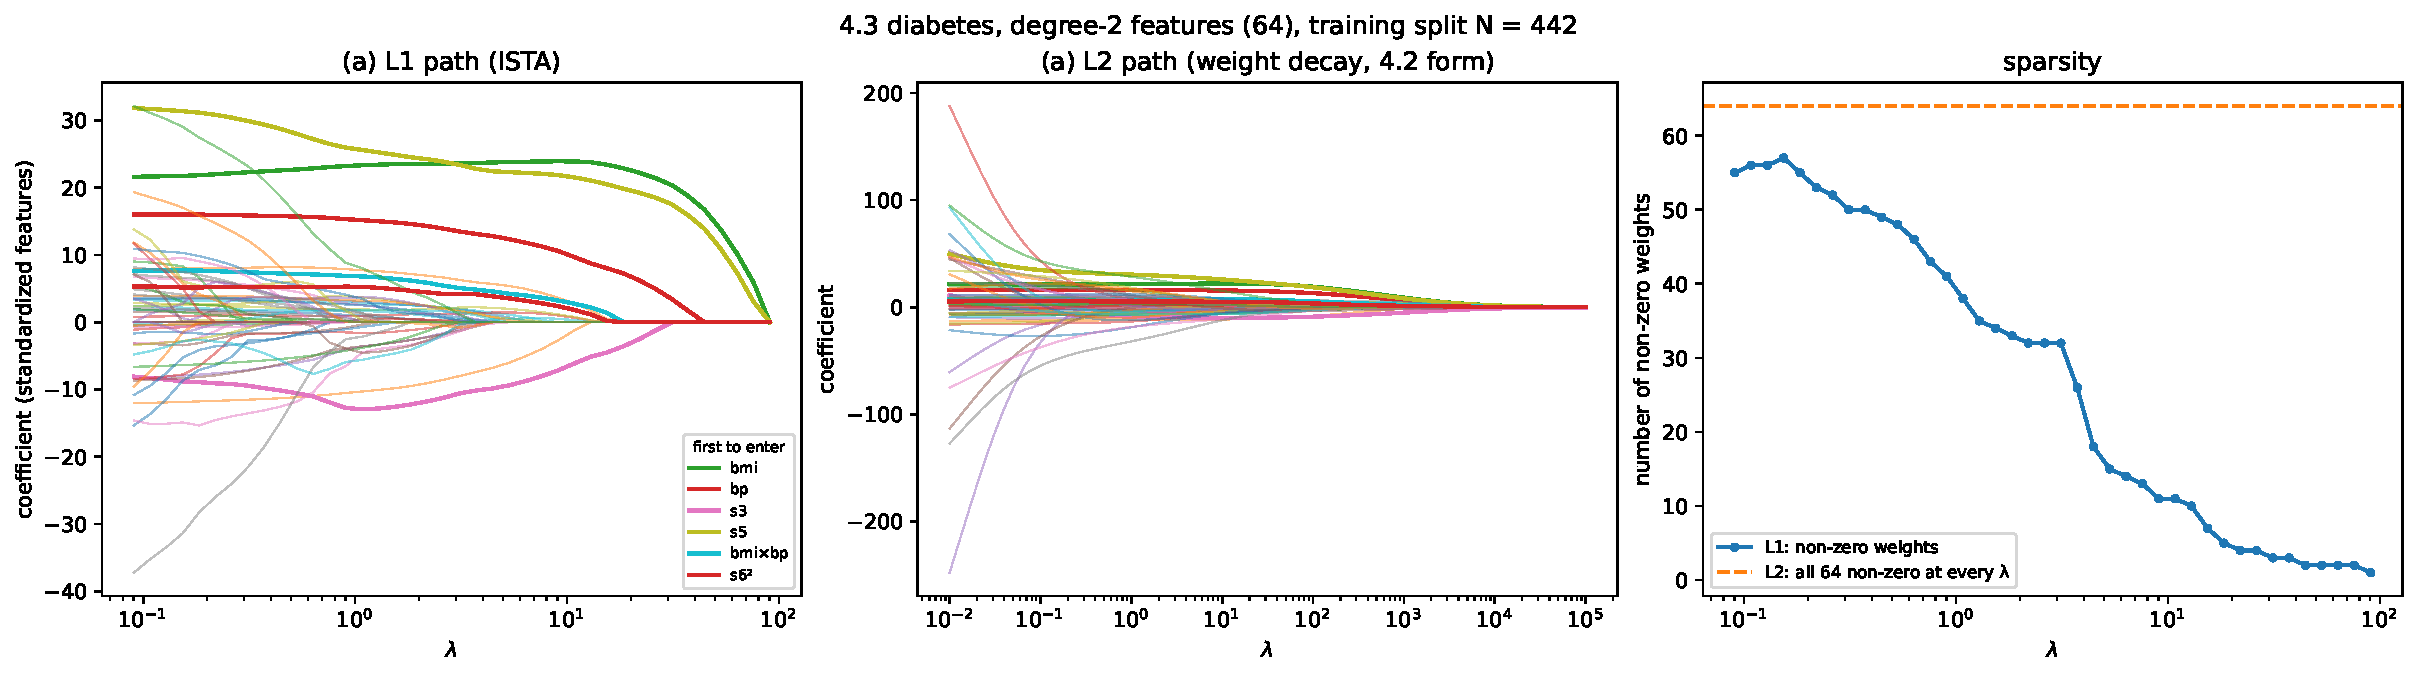
\includegraphics[width=0.64\textwidth]{fig_4_3a_paths}\label{fig:p4f}}\\
\subfloat[]{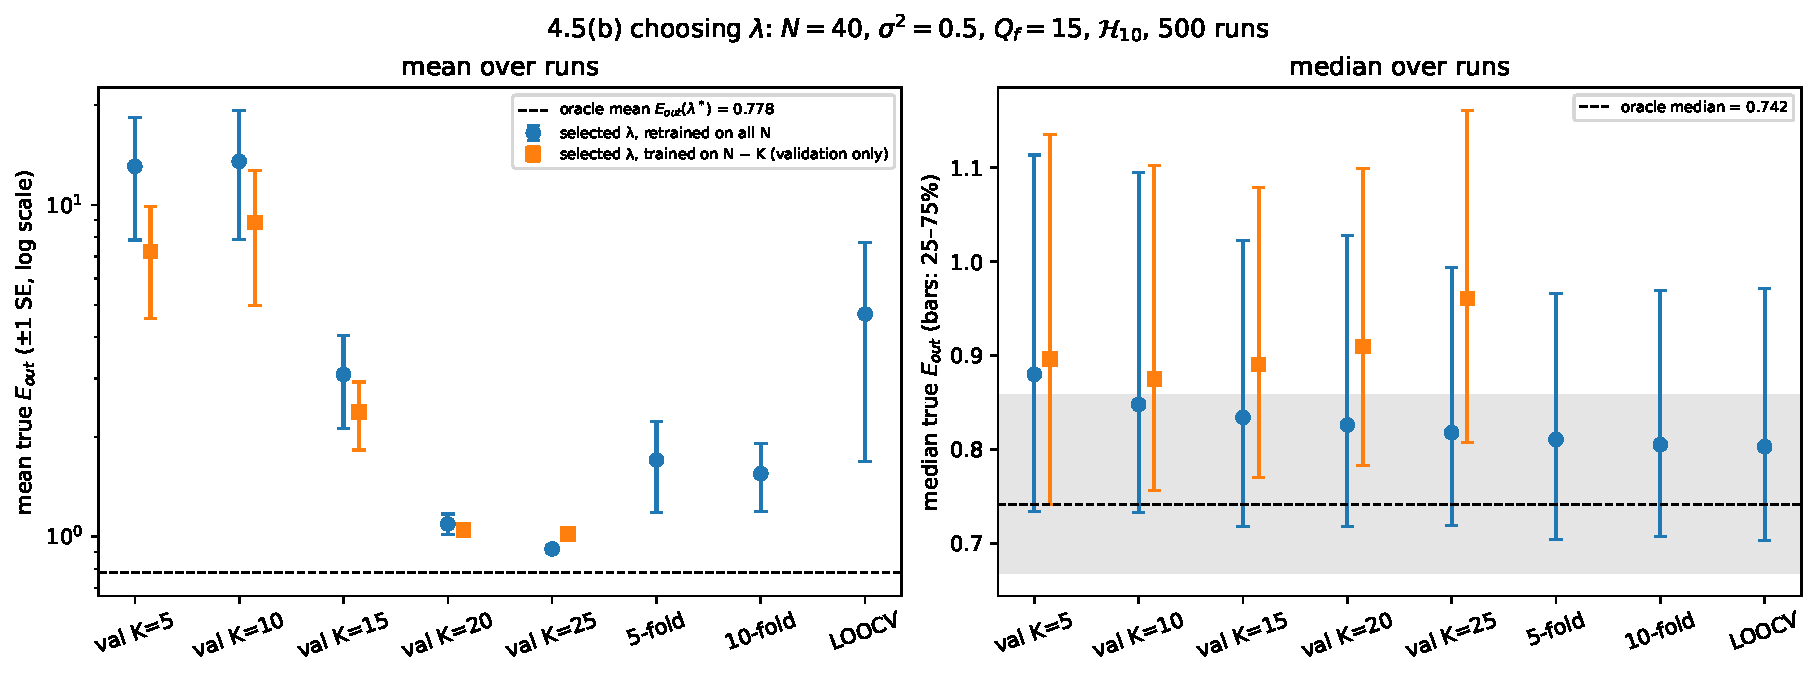
\includegraphics[width=0.49\textwidth]{fig_4_5b_selection}\label{fig:p4g}}\hfil
\subfloat[]{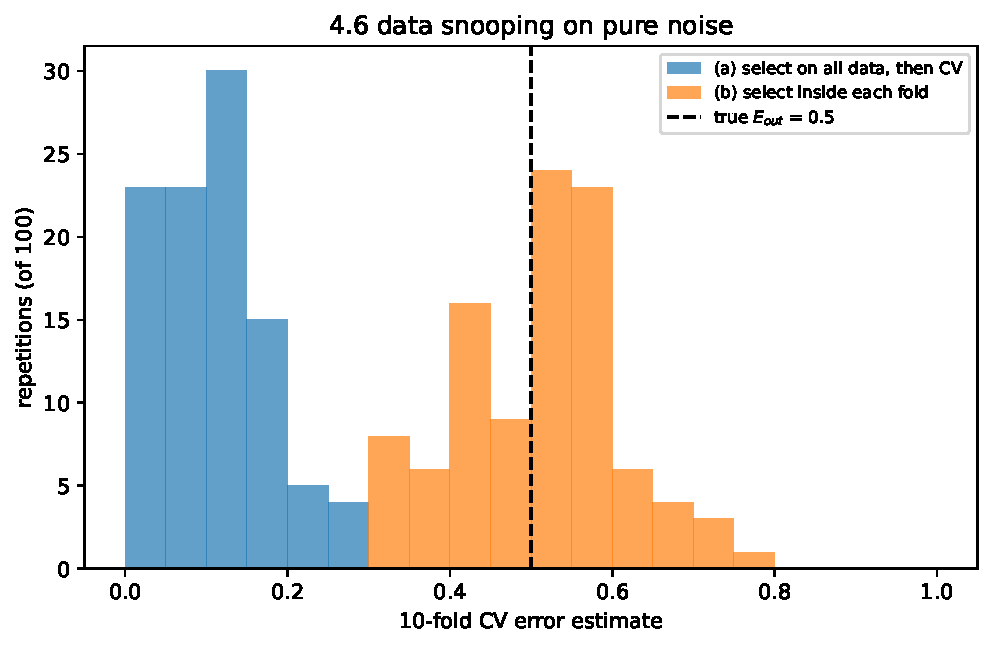
\includegraphics[width=0.31\textwidth]{fig_4_6_snooping}\label{fig:p4h}}
\caption{Part 4, continued. (a) Diabetes, degree-2 features: L1 and L2 paths and the number of non-zero weights. (b) Selecting $\lambda$ for weight decay ($N=40$, 500 runs): $\Eout$ of the selected model for each method against the oracle. (c) Data snooping on pure noise, 100 repetitions: 10-fold CV error with feature selection on all data and inside each fold.}
\label{fig:p4b2}
\end{figure*}

\textbf{Sparsity (4.3).} We selected 442 diabetes patients with degree-2 features and removed the $\mathrm{sex}^2$ feature because sex only has 2 values, leaving us with 64 standardized features. Decreasing the value of $\lambda$ below $\lambda_{\max}=90.3$, L1 admits weights one at a time (Fig.~\ref{fig:p4b2}(a)): 1 at $\lambda_{\max}$, 7 at $0.17\lambda_{\max}$, 55 at $0.001\lambda_{\max}$, starting with the BMI, followed by the serum triglycerides and blood pressure, whereas L2 admits all 64 non-zero weights. In a geometric sense, the corners of the L1 constraint region are on the axes, and a typical contour of $\Ein$ is likely to meet the L1 constraint region first at the corners. Algebraically, the soft-threshold in \eqref{eq:ista} is always zero when $|v_j|\le\eta\lambda$, while weight decay multiplies each direction by $s_i^2/(s_i^2+\lambda)$, which is never zero.

\textbf{Regularized logistic regression (4.4).} In the case of degree-2 features, there are 495 features and 100 training points, and the data are separable, so at $\lambda=0$ L-BFGS terminates at an arbitrary point (test error 0.062). In the case of 5-fold CV on the training points, $\lambda^*=0.631$ for L2 (test error 0.049) and $\lambda^*=0.0183$ for L1 (test error 0.041) are obtained, the latter selecting only 18 features out of 495: smoothness, concave points, texture, radius and area, the size and shape irregularities of malignant nuclei, which makes clinical sense~\cite{street1993}.

\textbf{Validation (4.5).} The closed form \eqref{eq:loocv} agrees with brute-force leave-one-out refits, with an unpenalized bias ($6\times10^{-13}$) and with a penalized one ($1.3\times10^{-12}$), over 62 values of $\lambda$. It requires only one SVD, rather than a separate fit for each point, so for 1600 points it is about a thousand times faster. Table~\ref{tab:cv} and Fig.~\ref{fig:p4b2}(b) compare the means of choosing $\lambda$ for weight decay. The worst performing method is a small validation set of 5 points, with median 0.880, while $K$-fold cross-validation and leave-one-out are closest to the oracle, with medians 0.80 to 0.81 against 0.74. The means are dominated by rare runs that select a small $\lambda$: in 10.8\% of the runs the 5-point validation set is above twice the error of the oracle, and in 5.0\% of the runs 10-fold cross-validation is. Lastly, the validation error of the selected model is optimistic in 65\% to 81\% of the runs: each individual validation error is unbiased, but we report the smallest of 62 noisy validation errors, and the smallest of many noisy numbers is biased low.

\begin{table}[!t]
\caption{Selecting $\lambda$ for weight decay, $N=40$, 500 runs (oracle: mean $0.778\pm0.007$, median $0.742$). Last column: share of runs with $\Eout$ above twice the oracle's.}
\label{tab:cv}
\centering\footnotesize
\begin{tabular}{lccc}
\toprule
Method & mean $\Eout$ & median & $>2\times$ oracle\\
\midrule
validation, $K=5$ & $13.1\pm5.2$ & 0.880 & 10.8\%\\
validation, $K=25$ & $0.918\pm0.024$ & 0.818 & 2.4\%\\
5-fold CV & $1.70\pm0.52$ & 0.811 & 4.6\%\\
10-fold CV & $1.55\pm0.36$ & 0.805 & 5.0\%\\
LOOCV & $4.69\pm3.00$ & 0.803 & 5.8\%\\
\bottomrule
\end{tabular}
\end{table}

\textbf{Data snooping (4.6).} The data are pure noise: 50 points, 1000 random features and labels from a coin flip, thus every classifier has a true error of $\Eout=0.5$. Choosing the 20 features most correlated with the labels on all the data, and only then cross-validating, gives an error of $0.103\pm0.006$, which is below 0.3 in all 100 repetitions (Fig.~\ref{fig:p4b2}(c)). Selecting them within each fold gives $0.508\pm0.010$. The selection step saw the validation points, so the chosen features correlate 0.37 with the labels, which is much higher than the typical 0.14. If we had fitted the standardization before splitting into folds, the same leak could have entered 3.5 and 4.4, so each fold refits its own.


\subsection{Part 5: The digits challenge}
\begin{figure*}[!t]
\centering
\subfloat[]{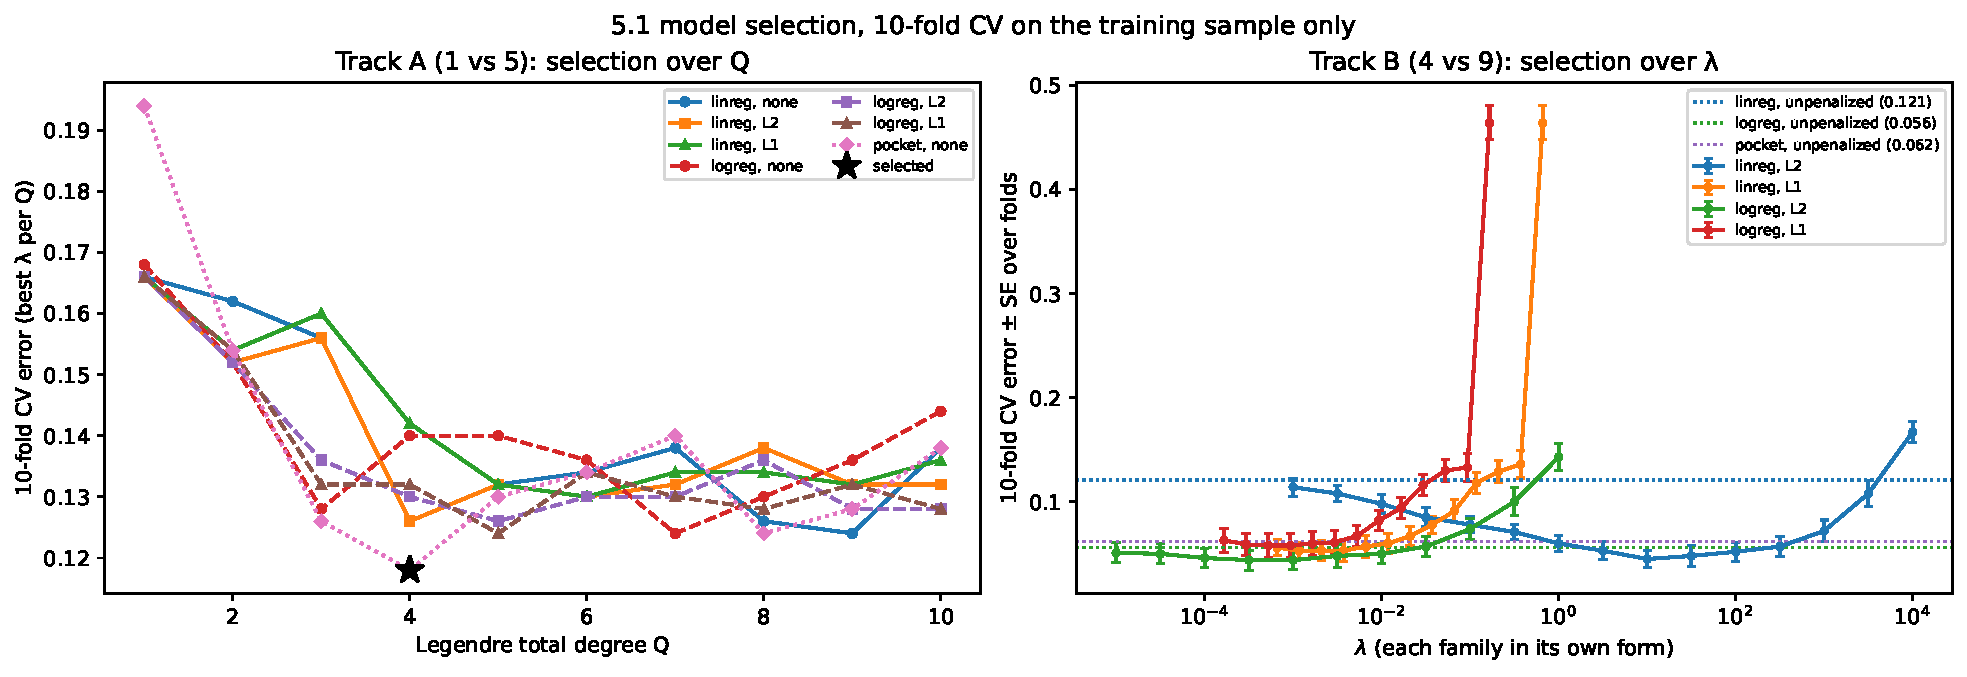
\includegraphics[width=0.46\textwidth]{fig_5_1_selection}\label{fig:p5a}}\hfil
\subfloat[]{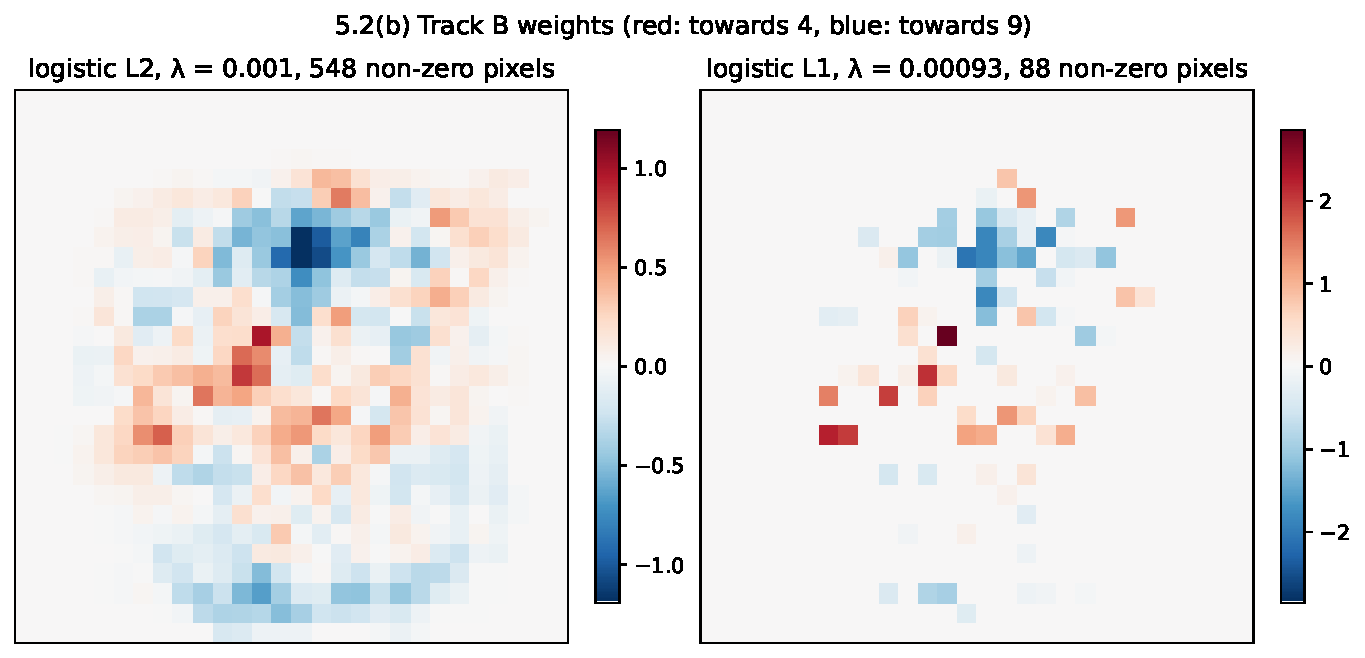
\includegraphics[width=0.22\textwidth]{fig_5_2b_track_b_weights}\label{fig:p5b}}
\caption{Part 5. (a) 10-fold CV error of every candidate: Track A against the Legendre degree $Q$, Track B against $\lambda$. (b) Track B weights as $28\times28$ images (red: towards 4, blue: towards 9), each at its own CV-selected $\lambda$.}
\label{fig:p5}
\end{figure*}

\textbf{Setup.} MNIST is divided into the first 60\,000 images as training data and the remaining 10\,000 images as test data. The Track A (1 vs 5) data set consists of 500 images with intensity and symmetry scaled to $[-1,1]$ within each fold and Legendre products up to total degree 10. Track B (4 vs 9) uses 1000 images and the 784 raw pixels. The candidates are Pocket (no penalty, always started at $\wlin$), linear regression and logistic regression, each with no penalty or with L2 or L1 over a grid of $\lambda$. We select the model with 10-fold CV on the training sample only, and if we have a tie, we select the simpler model.

\begin{table}[!t]
\caption{Part 5: the selected model per track, evaluated once on the test set.}
\label{tab:p5}
\centering\footnotesize
\begin{tabular}{lcc}
\toprule
 & Track A (1 vs 5) & Track B (4 vs 9)\\
\midrule
candidates & 550 & 55\\
selected & Pocket, $Q=4$ & logistic L2, $\lambda=10^{-3}$\\
CV error & $0.118\pm0.014$ & $0.044\pm0.009$\\
$\Ein$ / $E_{\mathrm{test}}$ & 0.122 / 0.141 & 0.011 / 0.041\\
test images & 2027 & 1991\\
95\% bound on $\Eout$ & $\le0.171$ & $\le0.072$\\
\bottomrule
\end{tabular}
\end{table}

\textbf{Test results.} The selected models are tested once (Table~\ref{tab:p5}), and for both tracks the 95\% Hoeffding margin is 0.030, with $M=1$. This is only so because the test set did not form part of the choice; if the test set had chosen from among the 550 candidates, it would have $M=550$, and repeated tuning would leave no fixed $M$. The test error of Track A is higher than its CV error because the winner is the best of 550 noisy estimates, as in 4.5.

\textbf{What the models learned.} In Track A the two features overlap: many 1s are thick and slanted, which gives them a 5's ink and breaks their symmetry, so each model stays near 12\% error. In Track B the L2 weights (Fig.~\ref{fig:p5}(b)) are smoothly distributed over the 548 pixels that carry ink in some training image: blue marks the pixels where a 9 closes its loop, and red the strokes of an open 4. L1 keeps 88 scattered pixels and is worse (CV 0.058), since neighbouring pixels contain the same evidence and L1 keeps one per group. The most confident errors are 4s with a closed top and 9s with an open loop.

\textbf{Comparing the tracks.} In Track B, regularization was important: with 785 weights for 900 points per fold, unpenalized least squares nearly memorized the data (CV 0.121), while ridge reached 0.045. In Track A all penalties are within 1 fold-SE of no penalty, so only the degree affects the error: with two overlapping features the model is bias-limited, and reducing the weights won't help with bias.


\section{Library comparison}\label{sec:lib}
Table~\ref{tab:lib} lists the agreement with scikit-learn~\cite{sklearn}. Differences have four sources:
\begin{itemize}
\item \textbf{Regularization convention.} \texttt{LogisticRegression} is regularized by default ($C=1$). It differs from our unpenalized fit by 1.11, but from our fit at $\lambda=1/(2N)$, its image under \eqref{eq:C}, by $1.4\times10^{-3}$.
\item \textbf{Tolerance.} With scikit-learn's default \texttt{tol}, the logistic weights differ by up to $9.3\times10^{-2}$ on breast cancer. With a tight tolerance the gap falls to $\le9.5\times10^{-5}$.
\item \textbf{Solver.} Iterative solvers agree to their stopping tolerances: GD to $10^{-9}$, L-BFGS to $8\times10^{-9}$, ISTA to $4\times10^{-9}$. The direct solvers agree to rounding.
\item \textbf{Scaling and intercept.} Both libraries fit the intercept unpenalized on the same standardized features, so neither contributes once matched. For Lasso and Ridge, the factors $\frac1{2N}$ and $\frac1N$ give $\lambda=2\alpha$ and $\alpha=\lambda$.
\end{itemize}

\begin{table}[!t]
\caption{Largest absolute weight difference from scikit-learn.}
\label{tab:lib}
\centering\footnotesize
\begin{tabular}{llc}
\toprule
Item & Comparison & $\max|\Delta w|$\\
\midrule
2.6 & \texttt{LinearRegression}, direct solvers & $\le1.2\times10^{-14}$\\
2.6 & \texttt{LinearRegression}, GD, L-BFGS & $\le8.3\times10^{-9}$\\
3.6 & \texttt{penalty=None}, simulated & $8.8\times10^{-10}$\\
3.6 & $C=1/(2N\lambda)$, breast cancer & $\le9.5\times10^{-5}$\\
4.3 & \texttt{Lasso}, $\alpha=\lambda/2$ (ISTA) & $\le4.2\times10^{-9}$\\
4.3 & \texttt{Ridge}, $\alpha=\lambda$ & $\le3.1\times10^{-12}$\\
\bottomrule
\end{tabular}
\end{table}

%==============================================================
\section{Discussion}\label{sec:disc}
\textbf{What we learned from simulated data that we could not from real data.} We selected the target and noise, so we knew the true out-of-sample error and could check the theory exactly: the in-sample error formula of 2.4 holds within 2.7 SEs, the analytic out-of-sample error matches the Monte Carlo estimate in our unit tests, and the closed-form leave-one-out error matches refitting to about 12 digits. Also, simulation allowed us to crank up stochastic and deterministic noise one at a time (4.1), and to display heavy tails near $N=d+1$, where means above $10^4$ were next to medians below 70, which only hundreds of fresh datasets can show. Finally, it measured a leak exactly: for actual data the snooped error of 4.6 would appear as a 90\%-accurate classifier, and only the known true error of 0.5 makes that apparent.

\textbf{What simulation couldn't teach us, real data did.} The prices of houses are capped and their features are correlated. Because breast cancer and MNIST pixels are linearly separable, unpenalized logistic regression does not have a finite solution there. Setting the threshold at 0.5 is a choice, not a default, because missing a cancer costs more than a false alarm. The textbook digit features are weak on both digit datasets. There was one test set for each real problem, so all the reported numbers have a Hoeffding margin of 0.03 to 0.13.

\clearpage
\begin{thebibliography}{00}
\bibitem{lfd} Y. S. Abu-Mostafa, M. Magdon-Ismail, and H.-T. Lin, \textit{Learning From Data}. AMLBook, 2012.
\bibitem{soudry2018} D. Soudry, E. Hoffer, M. S. Nacson, S. Gunasekar, and N. Srebro, ``The implicit bias of gradient descent on separable data,'' \textit{J. Mach. Learn. Res.}, vol. 19, no. 70, pp. 1--57, 2018.
\bibitem{beck2009} A. Beck and M. Teboulle, ``A fast iterative shrinkage-thresholding algorithm for linear inverse problems,'' \textit{SIAM J. Imaging Sci.}, vol. 2, no. 1, pp. 183--202, 2009.
\bibitem{odonoghue2015} B. O'Donoghue and E. Cand\`es, ``Adaptive restart for accelerated gradient schemes,'' \textit{Found. Comput. Math.}, vol. 15, no. 3, pp. 715--732, 2015.
\bibitem{sklearn} F. Pedregosa \textit{et al.}, ``Scikit-learn: Machine learning in Python,'' \textit{J. Mach. Learn. Res.}, vol. 12, pp. 2825--2830, 2011.
\bibitem{street1993} W. N. Street, W. H. Wolberg, and O. L. Mangasarian, ``Nuclear feature extraction for breast tumor diagnosis,'' in \textit{Proc. SPIE}, vol. 1905, 1993, pp. 861--870.
\end{thebibliography}

\section*{Contribution Statement}
\begin{center}\footnotesize
\begin{tabular}{p{0.36\columnwidth}p{0.54\columnwidth}}
\toprule
Part & Led by\\
\midrule
Part 0 (toolkit, tests) & N. Serik\\
Part 1 (Pocket PLA) & D. Toktybayev\\
Part 2 (linear regression) & D. Toktybayev\\
Part 3 (logistic regression) & D. Toktybayev\\
Part 4 (regularization) & N. Serik\\
Part 5 (MNIST) & N. Serik\\
Report and video & N. Serik, D. Toktybayev\\
\bottomrule
\end{tabular}
\end{center}
Both authors reviewed all parts of the submission and can explain any of them.

\end{document}
